\chapter{基于去偏成对损失的推荐算法研究}
\label{cha:fourthsection}
从成对比较中学习对比表示(Contrastive Representations)在自然语言处理、计算机视觉和信息检索等多个领域取得了显著的成功。基于成对学习的推荐算法也根植于这一范式。一个重要的问题是数据集普遍是positive-unlabeled,即负例未标注。这导致成对损失偏离了原始的优化目标,不再是完全监督数据下AUC风险的无偏估计。优化目标的偏离,不可避免地导致学到有偏的嵌入,从而对下游排序任务产生不利影响。本章致力于解决成对损失优化目标偏差的问题,得到了一种校正后的成对损失函数,称为去偏成对损失(Debiased Pairwise Loss, DPL)。DPL的核心思想是纠正由于伪负例引起的偏倚概率估计,从而修正梯度,使其逼近完全监督数据下成对损失的梯度。对五个公共数据集进行的实验研究验证了所提出的学习方法的有效性。

\section{引言}
成对损失BPR\cite{Steffen:2009:UAI}是个性化推荐领域最为广泛使用的优化目标之一。在完全监督数据下,成对损失的优势一方面在于,它根植于对比学习范式,编码样本之间的差异特征进行,而不是编码样本的像素级特征,通常能够获得更好的泛化性能~\cite{Wang:2020:ICML,McFadden:1974:FE,gutmann:2012:JMLR,Liu:2021:TKDE,Wang:2020:ICML}。另一方面的优势在于,在完全监督设置下,成对损失BPR\cite{Steffen:2009:UAI}是排序导向的优化目标,直接针对正例的得分高于负例这一排序目标进行优化。BPR损失可以类比于排序列比的AUC指标\cite{Steffen:2009:UAI},最小化BPR损失,也即最大化排序列表的AUC值。这个优良性质使得对比学习和个性化推荐任务具有一致性,因此BPR逐渐主导了从隐式反馈中学习排序的任务。

从单个成对比较来看,完全监督数据下的BPR的优化目标是“正例得分大于负例的似然”。从所有成对比较来看,完全监督数据下的BPR的优化目标是排序列表AUC风险的无偏估计。然而,用户通常只通过交互行为(点击、购买)提供正反馈,导致推荐系统的数据集是只有部分正例被标注的PU数据集。在使用PU数据集优化成对损失时,负例实际上是未标记样本。
这导致了成对损失偏离了原始的优化目标:从单个成对比较来看,使用正例和未标记样本建模的是一个偏倚的“正例得分大于负例的似然”(详细分析见本章\ref{2sec:2}节的介绍);从所有的成对比较来看,使用正例和未标记样本计算得到的BPR损失是一个有偏的AUC风险估计(详细分析见本章\ref{2sec:5}节的介绍)。成对损失优化目标的偏离,不可避免地导致模型学到有偏的用户物品特征,从而对下游排序任务产生不利影响。


%成对学习。成对学习已成为许多现代机器学习算法的基本组成部分,并在自然语言处理、图像和语音识别以及推荐系统等诸多领域取得了重大进展~\cite{Oord:2018:arxiv,Wang:2020:ICML,He:2020:CVPR,Steffen:2009:UAI}。在协同过滤中,成对学习被广泛应用于预测排序,其中最著名的方法是贝叶斯个性化排名(BPR)~\cite{Steffen:2009:UAI}。从统计角度来看,BPR最大化了观察到的正负样本的后验概率。从数值计算角度来看,BPR损失函数鼓励模型正例的得分高于负例。在嵌入空间中,BPR损失的目标是将正例的嵌入拉近到锚点(即用户),同时将负例的嵌入推离锚点。

针对这一问题,现有的研究主要从两个方向解决。第一类方法是负采样\cite{Steffen:2014:WSDM,Zhang:2013:SIGIR,Ding:2020:NIPS,Park:2019:WWW,Huang:2021:KDD,Ding:2019:IJCAI,Yang:2020:KDD},核心思想是采样用户不喜欢的真负例喂入模型训练,以避免上述优化目标偏离的问题。负采样可以分为两种类型:第一种是静态负采样,它使用固定的采样分布,利用与模型的训练状态无关的某种辅助信息,容易采样简单的样本,性能往往较差。此外,静态负采样严重依赖于辅助信息作为有效的监督信号,而这些监督信息在大多数场景下是难以获取的。第二种是动态负采样,使用与模型相关的信息(如预测得分)动态调整采样分布,旨在采样具有高得分或排名靠前的困难负样本,但容易遇到伪负例。此外,基于GPU批量计算的mini-batch训练与动态负采样不兼容。动态负采样通常需要额外的计算和存储开销,例如存储先前训练轮次的预测得分~\cite{Ding:2020:NIPS},或计算mini-batch之外样本的预测得分\cite{Zhang:2013:SIGIR,Steffen:2014:WSDM}。第二类方法是经验风险重写\cite{Su:2021:IJCAI,Christoffel:2016:ACML,Jain:2016:NIPS,Du:2015:ICML,Du:2014:NIPS},这类方法常见于PU学习(Positive-Unlabeled Learning)领域\cite{Jessa:2020:ML},核心思想是把未标注样本的分布进行全概率分解,重写基于PU数据计算得到的经验风险。然而,这类方法只适用于基于样本和标签构建的点式损失(Pointwise Loss),如均方误差(MSE),二元交叉熵(BCE),这类损失都是基于单个样本和标签构建的损失;成对损失则是在两个样本上构建的成对损失(Pairwise Loss),不涉及样本标签,现有的PU估计量难以向成对学习推广。

本章聚焦于没有任何辅助信息用于监督的最一般形式的隐式反馈数据,提出了一种在PU数据集下校正成对损失优化目标偏离的方法,从而为成对学习提供了一种修正后的损失函数,称为去偏成对损失(Debiased Pairwise Loss,DPL)。DPL的核心思想是修正使用未标记样本导致的概率估计偏差,从而修正梯度以近似完全监督数据的梯度。DPL不需要额外的辅助信息进行监督,也不需要过多的存储和计算开销。在严格保持相对于BPR线性复杂度的情况下,DPL在五个公开数据集上取得了更好的结果。

本章对推荐系统的成对学习优化目标研究做出了以下几个方面的贡献:(1)提出了有偏成对损失的估计校正方法,并提出了去偏成对损失DPL;(2)分析了去偏成对损失DPL的小样本性质,是排序列表AUC的无偏估计;(3)分析了去偏成对损失DPL的大样本性质,它是有监督设置下成对损失的一致估计。

\section{成对损失优化目标分析}\label{2sec:2}
将用户物品对$(u,i)$记为$\mathbf{x}$,其中$u\in \mathcal{U}$,$i\in \mathcal{I}$。令$\mathcal{X}= \{\mathbf x|u\in \mathcal{U}, i\in \mathcal{I}\}$表示包含所有用户物品对的样本空间,$\mathcal{Y} =\{-1,+1\}$表示类别标签,指示用户是否喜欢该物品。决策函数$g:\mathcal{X} \rightarrow \mathbb{R}$是一个实值函数,通常为用户物品表示的内积相似度或者余弦相似度,为每个交互分配一个预测的偏好水平$g(\mathbf x) \in \mathbb{R}$(预测评分在BPR中符号记为$\hat{x}_{ui}$,本章记为$g(\mathbf x)$有助于理论分析部分简化数学符号)。设正例的类条件密度表示为$p^+(\mathbf x) = p(\mathbf x|+1)$,负例的类条件密度表示为$p^-(\mathbf x) = p(\mathbf x|-1)$。

在理想的有监督标签的情况下,通过从正例类条件概率密度$p^+(\mathbf x)$抽样正例$\mathbf{x}^+$,从负例类条件概率密度$p^-(\mathbf x)$抽样正例$\mathbf{x}^-$,通过任意两个随机样本对$(\mathbf{x}^+, \mathbf{x}^-)$建模用户对正例$\mathbf{x}^+$的偏好大于负例$\mathbf{x}^-$的似然
\begin{align}\label{eq:bpr}
	\mathcal{L}_{BPR} &= - \mathbb{E}_{\substack{\mathbf x^+ \sim p^+(\mathbf x) \\ \mathbf x^- \sim p^-(\mathbf x^-)}} \log \sigma(g(\mathbf{x}^+) - g(\mathbf{x}^-)) \\
	&=  - \mathbb{E}_{\substack{\mathbf x^+ \sim p^+(\mathbf x) \\ \mathbf x^- \sim p^-(\mathbf x)}}\log \frac{1}{1+\exp(-g(\mathbf{x}^+) + g(\mathbf{x}^-))} \nonumber \\
	&=  - \mathbb{E}_{\substack{\mathbf x^+ \sim p^+(\mathbf x) \\ \mathbf x^- \sim p^-(\mathbf x^-)}}\log\frac{\exp(g(\mathbf{x}^+))}{\exp(g(\mathbf{x}^+))+\exp( g(\mathbf{x}^-))} \label{eq:infonce1}
\end{align}

值得注意的是,式\eqref{eq:infonce1}是贝叶斯个性化排名(BPR)损失的等价形式,它与噪声对比估计(NCE)损失\cite{Gutmann:2010:ICAIS}完全相同,而NCE损失是InfoNCE损失\cite{Oord:2018:arxiv}在只有一个负例(即N=1)的特殊情况。在协同过滤的场景中,用户和物品构成一个二分图,通常只选择用户嵌入作为锚点。在实际优化时,使用的是有限样本的经验形式。在有监督设置下,正例是从正例类条件密度中采样,表示为$\mathbf{x}^+ \in \mathcal{D}^+$,而负例是从负例类条件概率密度中采样的,表示为$\mathbf{x}^- \in \mathcal{D}^-$。因此,式\eqref{eq:bpr}的对应的经验估计可以表示为:
\begin{eqnarray}\label{eq:bpr_emp}
	\mathcal{L}_\text{BPR} =- \frac{1}{|\mathcal{D}^+|\times |\mathcal{D}^-|} \sum_{\mathbf{x}^+ \in \mathcal{D}^+}\sum_{\mathbf{x}^- \in \mathcal{D}^-} && \ln \sigma(g(\mathbf{x}^+) - g(\mathbf{x}^-))  - \lambda ||\Theta||^2,
\end{eqnarray}
其中,$\lambda ||\Theta||^2$ 是正则化项,用于平衡方差和偏差,避免过拟合。特别地,正则化项$\lambda ||\Theta||^2$等价于高斯分布的先验密度的对数,从而为式\eqref{eq:bpr_emp}提供了基于后验概率的解释。在原始的贝叶斯个性化排名(BPR)论文\cite{Steffen:2009:UAI}中,式\eqref{eq:bpr_emp}被解释为观测到的有序对的最大后验估计。

在实际中,由于缺乏标记的负例样本,在优化式\eqref{eq:bpr_emp}时,只能从未标记的数据中采样负例样本,表示为$\mathbf{x}^- \in \mathcal{D}^u$,导致以下偏倚的优化目标:
\begin{eqnarray}\label{eq:bpr_emp_biased}
	\mathcal{L} =- \frac{1}{|\mathcal{D}^+|\times |\mathcal{D}^u|} \sum_{\mathbf{x}^+ \in \mathcal{D}^+}\sum_{\mathbf{x} \in \mathcal{D}^u} && \ln \sigma(g(\mathbf{x}^+) - g(\mathbf{x})) - \lambda ||\Theta||^2,
\end{eqnarray}

接下来,考察单个成对比较的偏倚优化目标对学习到的模型参数$\Theta$的影响:
\begin{align}
	\frac{\partial \mathcal{L}}{\partial \Theta} &= \frac{\partial \mathcal{L}_\text{BPR}}{g(\mathbf{x})}\cdot\frac{g(\mathbf{x})}{\Theta}  \\
	&= [1-\sigma(g(\mathbf{x}^+) - g(\mathbf{x})) ]\cdot\frac{g(\mathbf{x})}{\Theta}  \label{eq:graident}
\end{align}
式\eqref{eq:graident}是微分链式法则的结果,其中第一项$[1-\sigma(g(\mathbf{x}^+) - g(\mathbf{x}))]$由损失函数的形式决定,第二项$\frac{g(\mathbf{x})}{\Theta}$由决策函数决定。对于固定的模型,第二项保持不变。

在式\eqref{eq:graident}的第一项中,实值sigmoid函数$\sigma(g(\mathbf{x}^+) - g(\mathbf{x})) \in [0,1]$被解释为用户偏好正例强于负例的似然\cite{Steffen:2009:UAI},是优化目标。然而,由于$\mathbf{x}$是未标记样本,它以$\tau^+$的先验概率是正样本,这导致了概率的偏倚估计。

图\ref{fig:event}提供了一个阐释性的例子说明为何使用正例-未标记数据对计算的值$\sigma(g(\mathbf{x}^+) - g(\mathbf{x}))$是一个偏倚的概率估计。“偏好正例强于负例的似然”,描述的是事件$\mathcal{A}_1(+,-)$的概率,这是优化目标。然而在PU数据集中,能获得的是正例-未标注样本对,导致成对学习优化的是事件$\mathcal{A}(+,u)$的概率。显然,事件$\mathcal{A}(+,u)$的概率和事件$\mathcal{A}_1(+,-)$的概率是不等价的,根据事件的可列可加性原理,事件$\mathcal{A}(+,u) = \mathcal{A}_1(+,-) + \mathcal{A}_2(+,+)$。理想优化目标$\mathcal{A}_1(+,-)$和实际优化目标$\mathcal{A}(+,-)$的不等价,导致了偏倚的“偏好正例强于负例”的概率估计,从而导致了有偏的最大似然/后验的优化目标。直观地说,偏倚的$\sigma(g(\mathbf{x}^+) - g(\mathbf{x}))$值会导致不正确的梯度大小${\partial \mathcal{L}_\text{BPR}}/{\partial \Theta}$,从而在执行随机梯度下降学习算法时导致不准确的用户-物品表示。
%%%%%%%%%%%%%%%%%%%%%%%%%%%%%%%%%%%%%%%%%%%%%%%%%%%%%%%%%%%
\begin{figure}[h!]
	\centering
	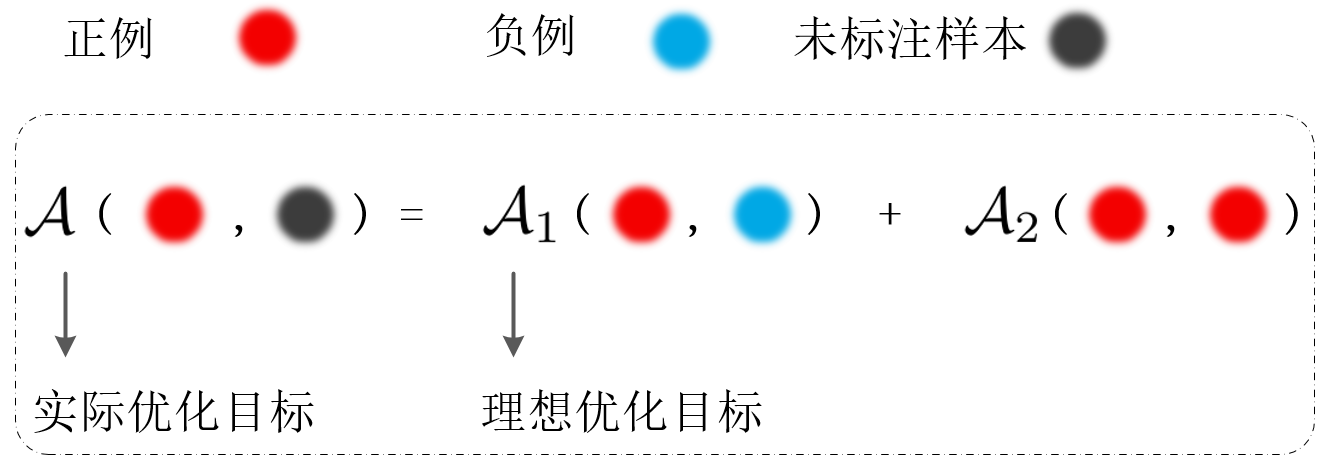
\includegraphics[width=0.6\textwidth]{4-event.png}
	\caption{成对损失优化目标偏差示意图} 
	\label{fig:event}
\end{figure}
%%%%%%%%%%%%%%%%%%%%%%%%%%%%%%%%%%%%%%%%%%%%%%%%%%%%%%%%%%%

为了使数学表达式保持简洁,本章定义一个映射$h: \mathcal{X}\times\mathcal{X} \rightarrow \sigma(g(\mathbf{x}_1) - g(\mathbf{x}_2))$,将两个样本映射到一个sigmoid函数。核心问题是,如何使用正例和未标注样本计算得到的概率值,估计使用正例和负例计算得到的概率值。具体而言,给定一组正例样本$\{\mathbf{x}_i\}_{i=1}^M$和一组未标记样本$\{\mathbf{x}_j\}_{j=1}^N$,目标是估计$h(\mathbf{x}^+,\mathbf{x}^-)$的值,以校正梯度,使其逼近完全监督数据下的梯度,从而提高学习到的用户-物品表示的泛化性能。

\section{去偏成对损失函数设计}
为了使用来自正例-未标记样本对来近似估计$h(\mathbf{x}^+,\mathbf{x}^-)$的值,首先建立正例-未标记样本对的联合分布$p_\textsc{pu}$与正例-负例样本对的联合分布$p_\textsc{pn}$之间的关系。

样本对的第一个样本,记为$\mathbf x_1$,是从正类条件概率$p^+(\mathbf x)$中确定性地抽取的,而第二个样本,记为$\mathbf{x}_2$,是从边缘分布$p(\mathbf{x})$中抽取的。因此,正例-未标记样本对的联合分布$p_\textsc{pu}$可以表示如下:
\begin{align}
	p_\textsc{pu}(\mathbf{x}_1, \mathbf{x}_2) &= p^+( \mathbf{x}_1) p( \mathbf{x}_2)  \label{eq:independent} \\
	&= p^+( \mathbf{x}_1) [p^+(\mathbf x_2) \tau^+ +p^-(\mathbf x_2)\tau^- ] \label{eq:full}\\
	&= \tau^+p^+( \mathbf{x}_1) p^+(\mathbf x_2) + \tau^-p^+( \mathbf{x}_1)p^-(\mathbf x_2) \label{eq:pnpp}
\end{align}
式\eqref{eq:independent}是由于$(\mathbf{x}_1, \mathbf{x}_2)$是独立抽样的,因此它们的联合概率分布为两个概率分布的乘积。式\eqref{eq:full}是通过将边际分布$p(\mathbf{x})$进行全概率分解。重新整理式\eqref{eq:pnpp},可以建立所需的正例-负例样本对的联合分布$p_\textsc{pn}(\mathbf{x}_1, \mathbf{x}_2)$与正例-未标记样本对的联合分布$p_\textsc{pu}(\mathbf{x}_1, \mathbf{x}_2)$之间的关系,表示为
\begin{eqnarray}\label{eq:jointpn}
	p_\textsc{pn}(\mathbf{x}_1, \mathbf{x}_2)  &=& p^+( \mathbf{x}_1)p^-(\mathbf x_2) \nonumber \\
	&=& \frac{1}{\tau^-}[p_{\textsc{pu}}(\mathbf{x}_1, \mathbf{x}_2)- \tau^+p^+( \mathbf{x}_1) p^+(\mathbf x_2)] \label{eq:pndist}
\end{eqnarray}

那么,$h(\mathbf x_1,\mathbf x_2)$相对正例-负例样本对的联合分布$p_\textsc{pn}(\mathbf{x}_1, \mathbf{x}_2)$上的期望,即理想的优化目标“用户喜欢正例$\mathbf{x}_1$优于负例$\mathbf{x}_2$”的概率期望值,可以计算如下:
\begin{align}
	&\mathbb{E}_{ p_\textsc{pn}(\mathbf{x}_1, \mathbf{x}_2)} h(\mathbf{x}_1,\mathbf{x}_2)\\
	&= \int_{\mathbf{x}_1}\int_{\mathbf{x}_2}   h(\mathbf{x}_1,\mathbf{x}_2) p_\textsc{pn}(\mathbf{x}_1, \mathbf{x}_2) d{\mathbf{x}_1}d{\mathbf{x}_2}\label{eq:pnh} \\
	&=\int_{\mathbf{x}_1}\int_{\mathbf{x}_2}   h(\mathbf{x}_1,\mathbf{x}_2) [\frac{1}{\tau^-}p_{\textsc{pu}}(\mathbf{x}_1, \mathbf{x}_2)- \frac{\tau^+}{\tau^-}p^+( \mathbf{x}_1) p^+(\mathbf x_2)]d{\mathbf{x}_1}d{\mathbf{x}_2} \label{eq:pn}\\
	&=\int_{\mathbf{x}_1}\int_{\mathbf{x}_2}   h(\mathbf{x}_1,\mathbf{x}_2) [\frac{1}{\tau^-}p_{\textsc{pu}}(\mathbf{x}_1, \mathbf{x}_2) d{\mathbf{x}_1}d{\mathbf{x}_2}- \int_{\mathbf{x}_1}\int_{\mathbf{x}_2} \frac{\tau^+}{\tau^-}p^+( \mathbf{x}_1) p^+(\mathbf x_2)]d{\mathbf{x}_1}d{\mathbf{x}_2} \\
	&= \frac{1}{\tau^-}\mathbb{E}_{ p_\textsc{pu}(\mathbf{x}_1, \mathbf{x}_2)} h(\mathbf{x}_1,\mathbf{x}_2) -\frac{\tau^+}{\tau^-} \mathbb{E}_{ p_\textsc{pp}(\mathbf{x}_1, \mathbf{x}_2)} h(\mathbf{x}_1,\mathbf{x}_2) \label{eq:expec}
\end{align}
其中,式\eqref{eq:pn}是把公式\eqref{eq:pndist}中计算到的$p_\textsc{pn}(\mathbf{x}_1, \mathbf{x}_2)$带入到式\eqref{eq:pnh}得到的结果。式\eqref{eq:expec}的第一项表示$ h(\mathbf{x}_1,\mathbf{x}_2)$在$ p_\textsc{pu}(\mathbf{x}_1, \mathbf{x}_2)$分布下的期望值,可以使用$N$个正例-未标记样本对$\{(\mathbf{x}^+_n,\mathbf{x}_n)\}_{n=1}^N$进行经验估计:
\begin{eqnarray}
	\mathbb{E}_{ p_\textsc{pu}(\mathbf{x}_1, \mathbf{x}_2)} h(\mathbf{x}_1,\mathbf{x}_2) &=& \frac{1}{N} \sum_{n=1}^{N} h(\mathbf{x}^+,\mathbf{x}_n)\label{eq:epu},
\end{eqnarray}
式\eqref{eq:expec}的第二项表示$ h(\mathbf{x}_1,\mathbf{x}_2)$在$ p_\textsc{pp}(\mathbf{x}_1, \mathbf{x}_2)$分布下的期望值,可以使用额外的$M$个正例-正例样本$\{(\mathbf{x}^+_m,\mathbf{x}'_m)\}_{m=1}^M$进行经验估计
\begin{eqnarray}
	\mathbb{E}_{ p_\textsc{pp}(\mathbf{x}_1, \mathbf{x}_2)} h(\mathbf{x}_1,\mathbf{x}_2)  &=& \frac{1}{M} \sum_{m=1}^{M} h(\mathbf{x}^+,\mathbf{x}_m^{\prime})\label{eq:epp}.
\end{eqnarray}

将式\eqref{eq:epu}和式\eqref{eq:epp}代入式\eqref{eq:expec},可以得到理想的优化目标“用户喜欢正例$\mathbf{x}_1$优于负例$\mathbf{x}_2$”的概率期望值的经验估计:
\begin{eqnarray}\label{eq:est}
	\hat{P}_\textsc{pn} = \frac{1}{N\tau^-}
	\sum_{\mathbf{x} \in \mathcal{D}^u}h(\mathbf{x}^+,\mathbf{x})  - \frac{\tau^+}{M\tau^-}\sum_{\mathbf{x}^\prime\in \mathcal{D}^+}h(\mathbf{x}^+, \mathbf{x}^\prime)
\end{eqnarray}
其中,$h: \mathcal{X}\times\mathcal{X} \rightarrow \sigma(g(\mathbf{x}_1) - g(\mathbf{x}_2))$是将两个样本映射到一个sigmoid函数,$g(\mathbf{x}_1)$是用户$u$对某个物品$i$相似度评分,即为$\hat{x}_{ui}$,通常为余弦相似度或者内积相似度。那么上式可以写为熟悉的形式:
\begin{eqnarray}\label{eq:est1}
	\hat{P}_\textsc{pn} = \frac{1}{N\tau^-}
	\sum_{j \in \mathcal{I}_u^-}\sigma(\hat{x}_{ui}-\hat{x}_{uj})  - \frac{\tau^+}{M\tau^-}\sum_{i^\prime \in \mathcal{I}_u^+}h(\hat{x}_{ui} - \hat{x}_{ui^\prime})
\end{eqnarray}
其中,$\mathcal{I}_u^-$是用户$u$未交互物品,$\mathcal{I}_u^+$是用户$u$已交互物品。式\eqref{eq:est1}的第一项,描述的是把所有未标记样本当作负样本,即使用正例-未标注样本对计算的$AUC$风险,记为$AUC_\textsc{pu}$。式\eqref{eq:est}中的第二项,即使用正例-正例样本对计算的校正项,用以校正未标记样本中伪负样本而导致的偏倚似然估计。

%%%%%%%%%%%%%%%%%%%%%%%%%%%%%%%%%%%%%%%%%%%%%%%%%%%%%%%%%%%
\begin{figure*}[h!]
	\centering
	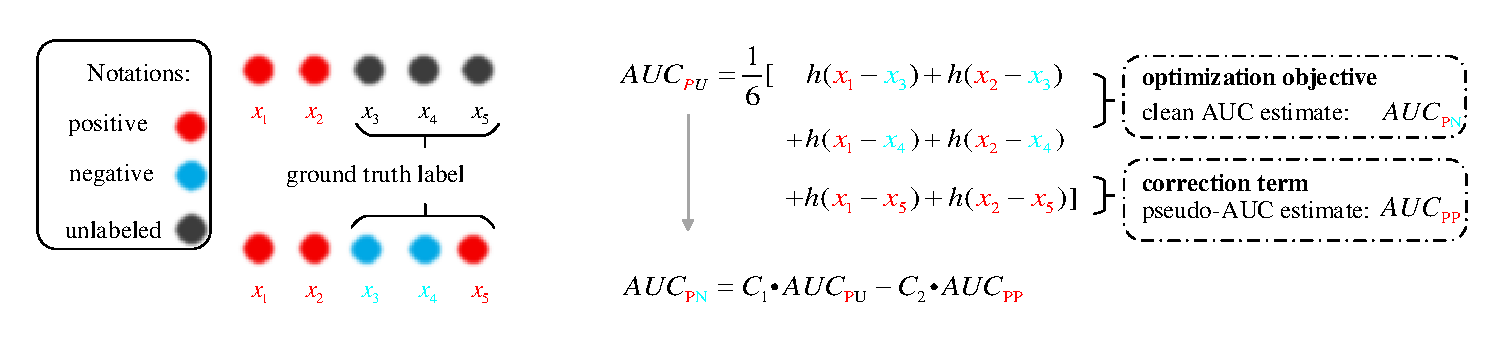
\includegraphics[width=\textwidth]{4-unbiasedAUC.pdf}
	\caption{去偏成对损失的示意图} 
	\label{fig:auc}
\end{figure*}
%%%%%%%%%%%%%%%%%%%%%%%%%%%%%%%%%%%%%%%%%%%%%%%%%%%%%%%%%%%

有了式\eqref{eq:est1}给出的优化目标“用户对正例$\mathbf{x}_1$的偏好强于负例$\mathbf{x}_2$”的概率,可以很容易进行极大似然估计。按照BPR的做法,本章也最大化对数似然,最大化式\eqref{eq:est}的对数,以优化去偏的成对损失(Debiased Pairwise Loss,DPL)。
%\begin{eqnarray}\label{eq:dpl}
%	\mathcal{L}_\textsc{dpl}=- \frac{1}{|\mathcal{D}^+|\times |\mathcal{D}^u|} \sum_{\mathbf{x}^+ \in \mathcal{D}^+}\sum_{\mathbf{x} \in \mathcal{D}^u} && \ln \hat{P}_\textsc{pn}.
%\end{eqnarray}

DPL与BPR的关键区别在于计算公式~\eqref{eq:est}中\textit{正样本优于负样本的似然概率$\hat{P}_\textsc{pn}$}的计算方式。公式中的第一项使用了正负样本对的方法,类似于BPR,但是加入了一个额外的校正项,用于抵消由于将误分类的负样本包含在无标签集合中造成的估计偏差。在公式~\eqref{eq:est}中,从正正样本对中计算的校正项可能看起来有些奇怪,但是AUC优化为这个校正项的来源提供了直观的解释,参考图~\ref{fig:auc}。

考虑一个正例-未标记的数据集,其中$\{x_1, x_2\}$是正例,$\{x_3, x_4, x_5\}$是未标记样本。这三个未标记样本中,$\{x_3, x_4\}$是真负例,$\{x_5\}$是正例,但是在训练过程中,无法访问未标记样本$\{x_3, x_4, x_5\}$的真实标签。把未标记样本$\{x_3, x_4, x_5\}$都当作负例,和两个正例$\{x_1, x_2\}$计算得到的PU数据下的$AUC$风险$AUC_\textsc{pu}$共2x3=6项,如图\ref{fig:auc}所示。其中,前4项是使用正例-负例(PN)数据对计算的“干净”$AUC$估计,是理想的优化目标,表示为$AUC_\textsc{pn}$。后两项是使用正例-正例(PP)数据对计算的伪$AUC$估计,表示为$AUC_\textsc{pp}$。

可以看到,使用PU数据集计算的$AUC$风险(实际优化目标),包含了最后的两项伪AUC估计,导致成对损失偏离了原始优化目标,从而是一个有偏的排序列表$AUC$估计。为了得到“干净”的$AUC$风险,应该从实际优化目标$AUC_\textsc{pu}$中减去正例-正例对计算的$AUC_\textsc{pp}$。而减去的补偿项目,正是由式\eqref{eq:est}的第二项基于正例-正例对计算的伪$AUC$估计。



DPL与先前的去偏差对比损失方法DCL\cite{Chuang:2020:NIPS}之间的区别在于它们如何校正偏倚的概率估计。在公式~\eqref{eq:est}中,DPL直接校正了偏置的概率估计;而DCL通过调整真负样本的得分间接校正它们(如公式~\eqref{eq:DCL}所示)。这种去偏差机制的差异导致DPL优化了AUC风险的无偏估计(如引理~\ref{lemma:auc}所示),而DCL\cite{Chuang:2020:NIPS}则不具备这种小样本性质。这个优势主要源于在成对学习设置中,只有一个无标签样本,可以枚举出无标签样本的所有可能标签情况,如图~\ref{fig:event}所示。相比之下,在具有$N$个无标签样本的对比损失情况下,共有$2^N$种可能的标签配置,使得枚举无标签样本的可能标签配置变得困难。
\section{算法实现与时间复杂度分析}
\subsection{算法实现}
在使用BPR损失进行训练时,对于每个$(u,i)$对,需要一个负样本$j$,从而形成一个$(u,i,j)$的训练三元组。为了校正成对损失的偏差,DPL损失要求对于每个$(u,i)$对,额外采样$M\geq 1$个正例和$N\geq1$个负例。遵循与BPR相同的数据条目格式,每个优化DPL损失的数据条目被组织为$(u,i,i_1,i_2,\cdots,i_M,j_1,j_2,\cdots,j_N)$,其中,$(i_1,i_2,\cdots,i_M,j_1,j_2,\cdots,j_N)$是额外的M个正例和N个未标记样本。这可以通过重写\verb|Dataloader|的\verb|collate_fn|函数,实现将一个批量大小为bs个交互$(u,i)$的mini-batch数据,改写为含有bs个数据条目为$(u,i,i_1,i_2,\cdots,i_M,j_1,j_2,\cdots,j_N)$的mini-batch数据。算法伪码见算法\ref{4Alg2:1}所示。
\begin{algorithm}[!]
	\counterwithin{algorithm}{chapter}
	\SetKwInput{KwIn}{输入}  %<---细节与重点
	\SetKwInput{KwOut}{输出}  %<---细节与重点
	\SetAlgoLined
	\small
	\caption{Pytorch的collate\_fn函数重写}\label{4Alg2:1}
	\KwIn{含有bs个交互$(u,i)$的mini-batch数据$\mathcal{R}$,批量大小bs,物品集合$\mathcal{I}$,用户正例集合$\mathcal{I}_u^+$。}
	\KwOut{含有bs个条目为$(u,i,i_1,i_2,\cdots,i_M,j_1,j_2,\cdots,j_N)$的mini-batch数据$\mathcal{R}\prime$。}
	\For{$(u,i) \in \mathcal{R}$}
	{
		~~从正例集合$\mathcal{I}_u^+$中随机采样M个正例$i_1,i_2,\cdots,i_M$;\\
		从未标注样本集合$\mathcal{I}_u^+$中随机采样N个未标注样本$j_1,j_2,\cdots,j_N$;\\
		将交互$(u,i)$、M个正例、N个负例拼接为1个数据条目;\\
		将该数据条目添加到$\mathcal{R}\prime$中;
	}
	\KwResult{含有bs个条目为$(u,i,i_1,i_2,\cdots,i_M,j_1,j_2,\cdots,j_N)$的mini-batch数据$\mathcal{R}\prime$。}
\end{algorithm}

因此,每个mini-batch数据结构组织如下:
\begin{eqnarray}\label{eq:mini}
	\text{batch size}\left\{ \left[\begin{array}{cccccccccc}
		u^{1} & {i}   &i_{1} & i_{2} & \ldots &i_{M} &   j_{1}& j_{2} & \ldots &j_{N} \\
		u^{2} & i & i_{1}& i_{2} & \ldots &i_{M} &  j_{1}& j_{2} & \ldots &j_{N} \\
		\vdots & \vdots & \vdots & \vdots &\ddots & \vdots & \vdots & \vdots & \ddots & \vdots \\
		u^{bs} & i & i_{1}& i_{2} & \ldots &i_{M} &  j_{1}& j_{2} & \ldots &j_{N} 
	\end{array}\right]\right.
\end{eqnarray}
每个数据条目包括N个未标记的样本$j_1,j_2,\cdots,j_N$,可以计算相应的N个预测得分 $\hat{x}_{j}^1,\hat{x}_{j}^2,\cdots,\hat{x}_{j}^N$。对于给定的正例样本 $(u,i)$,其得分为 $\hat{x}_i$,可以基于N个负例样本的预测得分得到N个PU概率值。因此,基于mini-batch估计的PU概率值为
\[\hat{P}_\textsc{pu} = \frac{1}{N} \sum_{n=1}^{N}\sigma (\hat{x}_i - \hat{x}_{j}^n)\]
类似地,可以计算出M个正例$i_1,i_2,\cdots,i_M$ 对应的M个预测得分 $\hat{x}_{i}^1,\hat{x}_{i}^2,\cdots,\hat{x}_{i}^M$,相应地,计算PP概率值估计为:
\[\hat{P}_\textsc{pp} = \frac{1}{M} \sum_{m=1}^{M}\sigma (\hat{x}_i - \hat{x}_{i}^m)\]

因此,经过校正后的理想的优化目标为:
\[\hat{P}_\textsc{pn} = \frac{1}{\tau^-}
\hat{P}_\textsc{pu} - \frac{\tau^+}{\tau^-}\hat{P}_\textsc{pp} \]
和BPR一样最大化对数似然,只需要对上式求对数后,执行梯度下降。去偏成对学习算法伪码见算法\ref{4-Alg:2}。
%\begin{algorithm}[!]
%	\small
%	\caption{去偏成对学习算法(DPL)伪代码}\label{4-Alg:2}
%	\KwIn{Mini-batch数据 $\mathcal{R}\prime$如式\eqref{eq:mini}所示, 评分函数$s(\cdot)$,额外正例数量M,额外负例数量N,正例类先验$\tau^+$,批量大小bs。}
%	\KwOut{模型参数$\Theta \in \mathbb{R}^d$}
%	\For{迭代次数$t= 1,2,...,T$}{
%		~~从训练集中抽样一个mini-batch数据 $\mathcal{R}\prime$如式\eqref{eq:mini}所示;\\
%		正向计算评分scores = s ($\mathcal{R}\prime$);   \# [bs * (1+M+N)] \\
%		pos\_scores = scores[: , : M+2];   \# [bs * (1+M)]  \\
%		neg\_scores = scores[: , M+2:]; \# [bs * N] \\
%		pu\_prob = sigmoid(pos\_scores[:, 0:1] - neg\_scores); \# [bs*N] \\ 
%		pp\_prob = sigmoid(pos\_scores[:, 0:1] - pos\_scores[:,1:]);  \# [bs*M]  \\
%		pn\_prob = pu\_prob.mean(dim=-1)/(1-tau) - $\tau^+ \cdot$ pp\_prob.mean(dim=-1)/(1-tau); \#[bs, ] \\
%		dpl\_loss = - log (pn\_prob).mean(); \\
%		根据dpl\_loss相对于$\Theta$的梯度更新参数;
%	}
%	\KwResult{用户和物品表示$\Theta$。}
%\end{algorithm}

\begin{algorithm}
	\counterwithin{algorithm}{chapter}
	\SetKwInput{KwIn}{输入}  %<---细节与重点
	\SetKwInput{KwOut}{输出}  %<---细节与重点
	\SetAlgoLined
	\small
	\caption{去偏成对学习算法(DPL)伪代码}\label{4-Alg:2}
	\KwIn{Mini-batch数据 $\mathcal{R}\prime$如式\eqref{eq:mini}所示, 评分函数$g(\cdot)$,额外正例数量M,额外负例数量N,正例类先验$\tau^+$。}
	\KwOut{模型参数$\Theta \in \mathbb{R}^d$。}
	~~计算正例相似度评分$g(u,i)$为$\hat{x}^+_{ui}$;\\
	计算M个额外正例相似度评分$\{\hat{x}^+_m\}_{m=1}^M$;\\
	计算N个未标注样本相似度评分$\{\hat{x}_n\}_{n=1}^N$;
	
	\For{$n = 1,2,\cdots, N$}{
		$p^\text{pu}_n =\sigma(\hat{x}^+_{ui} - \hat{x}_n) $ \textbackslash\textbackslash~~~$\textsc{pu}$概率值
	}
	
	\For{$m = 1,2,\cdots, M$}{
		$p^\text{pp}_m =\sigma(\hat{x}^+_{ui} - \hat{x}^+_m) $ \textbackslash\textbackslash~~~$\textsc{pp}$概率值
	}
	~~计算$\textsc{pu}$概率均值$p^\text{pu}_\text{mean} = \frac{1}{N}\sum_{n=1}^{N}p^\text{pu}_n$;\\
	计算$\textsc{pp}$概率均值$p^\text{pp}_\text{mean} = \frac{1}{M}\sum_{m=1}^{M}p^\text{pp}_m$;\\
	计算$\textsc{pn}$概率估计$p^\text{pn} = \frac{1}{\tau^-}p^\text{pu}_\text{mean}  - \frac{\tau^+}{\tau^-}p^\text{pp}_\text{mean}$;\\
	$\text{dpl}_\text{loss}   = - \log (p^\text{pn})$;\\
	根据dpl\_loss相对于$\Theta$的梯度更新参数;

	\KwResult{模型参数$\Theta \in \mathbb{R}^d$。}
\end{algorithm}
\subsection{时间复杂度分析}
首先分析基线方法BPR的复杂度,与评分函数有关。这里,以维度为$d$的矩阵分解作为示例,这个分析可以很容易地推广到其他模型。给定一个批量大小为$bs$的$(u,i,j)$的训练三元组,前向传播计算相似度评分过程中,涉及到总共$2\times bs$个物品得分预测,因此时间复杂度为$\mathcal O(2 bs\times d)$。在反向传播更新参数过程中,由于共$bs$个$(u,i,j)$三元组,最多更新$3 \times bs$个用户和物品嵌入。因此,BPR的一个Mini-batch数据涉及总共$5bs\times d$次操作,时间复杂度为$\mathcal O(bs\times d)$。类似地,对于DPL,一个小批量数据涉及到总共$(M+N+1)\times bs$个评分计算和$(M+N+2)\times bs$个嵌入更新,涉及总共$(2M+2N+3)\times bs\times d$个操作,时间复杂度为$\mathcal O(bs\times d)$,因为在实践中通常将$M$和$N$设置为小的常数,例如$M=3$和$N=3$。特别地,当$M=0$且$N=1$时,DPL涉及的操作次数与BPR相同。因此,相对于BPR,DPL具有严格的线性复杂度,没有任何mini-batch数据之外的计算或者存储开销。而前面的负采样算法,由于涉及计算用户每个训练三元组中用户$u$对应的评分向量,从而产生了mini-batch数据之外的计算开销。而推荐中,物品数量通常非常大,导致了时间复杂度的增加。

\section{去偏成对损失的理论分析}\label{2sec:5}
\subsection{小样本性质}
DPL的主要思想是改进使用正例-未标记数据对(PU)计算的偏倚概率$P_\textsc{pu}$。通过采样额外的正例和负例样本进行来估计式\eqref{eq:est}所给出的理想优化目标“用户喜欢正例$\mathbf{x}_1$优于负例$\mathbf{x}_2$”的概率$\hat P_\textsc{pn}$,然后用其替代原始的偏倚概率估计$P_\textsc{pu}$。为了证明$\hat P_\textsc{pn}$是一个良好的估计量,首先证明$\hat P_\textsc{pn}$是排序列表$AUC$风险的无偏估计。
\begin{lemma}\label{lemma:auc} 设正例$\mathbf{x}^+$是从正例的类条件概率分布$p^+(\mathbf{x})$独立采样的样本, 未标注样本$\mathbf{x}$是从边际分布$p(\mathbf{x}) = \tau^+ p^+(\mathbf{x})+ \tau^- p^-(\mathbf{x})$独立采样的样本。 那么公式~\eqref{eq:est}给出的$\hat P_\textsc{pn}$是无偏的AUC风险估计:
	\[\mathbb{E}\hat P_\textsc{pn} = R_{AUC}\]
	\begin{proof}
		\begin{align}
			\mathbb{E}\hat P_\textsc{pn} &=\int_{\mathbf{x}^+} [\frac{1}{N\tau^-}
			\sum_{\mathbf{x} \in \mathcal{D}^u} \mathbb{E}_{\mathbf{x}\sim p}h(\mathbf{x}^+,\mathbf{x}) - \frac{\tau^+}{M\tau^-}\sum_{\mathbf{x}^\prime\in \mathcal{D}^+}\mathbb{E}_{\mathbf{x}^\prime \sim p^+}h(\mathbf{x}^+, \mathbf{x}^\prime)]p^+(\mathbf{x}^+)d\mathbf{x}^+ \\
			&=\int_{\mathbf{x}^+} [\frac{1}{\tau^-}
			\mathbb{E}_{\mathbf{x}\sim p}h(\mathbf{x}^+,\mathbf{x}) - \frac{\tau^+}{\tau^-}\mathbb{E}_{\mathbf{x}^\prime \sim p^+}h(\mathbf{x}^+, \mathbf{x}^\prime)]p^+(\mathbf{x}^+)d\mathbf{x}^+ \label{eq:unbiasauc}.
		\end{align}
由于
		\begin{align}
			&\frac{1}{\tau^-}\mathbb{E}_{\mathbf{x}\sim p}h(\mathbf{x}^+,\mathbf{x}) - \frac{\tau^+}{\tau^-}\mathbb{E}_{\mathbf{x}^\prime\sim p^+}h(\mathbf{x}^+, \mathbf{x}^\prime)\nonumber \\
			&=\frac{1}{\tau^-} \int_\mathbf{x}h(\mathbf{x}^+,\mathbf{x})p(\mathbf{x})d\mathbf{x} - \frac{\tau^+}{\tau^-} \int_\mathbf{x^\prime}h(\mathbf{x}^+, \mathbf{x}^\prime)p^+(\mathbf{x}^\prime)d\mathbf{x^\prime} \nonumber \\
			&=\frac{1}{\tau^-} \int_\mathbf{x}h(\mathbf{x}^+,\mathbf{x})[\tau^+p^+(\mathbf{x}) + \tau^-p^-(\mathbf{x}) ]d\mathbf{x} - \frac{\tau^+}{\tau^-} \int_\mathbf{x^\prime}h(\mathbf{x}^+, \mathbf{x}^\prime)p^+(\mathbf{x}^\prime)d\mathbf{x^\prime}  \label{eq:marginal} \\
			&= \int_\mathbf{x}h(\mathbf{x}^+,\mathbf{x})p^-(\mathbf{x})d\mathbf{x} \label{eq:variable} \\
			&= \int_\mathbf{x^-}h(\mathbf{x}^+,\mathbf{x}^-)p^-(\mathbf{x}^-)d\mathbf{x}^- \label{eq:pmin} 
		\end{align}
其中,公式~\eqref{eq:marginal}是通过边际分布的全概率分解$p(\mathbf{x})= \tau^+p^+(\mathbf{x}) + \tau^-p^-(\mathbf{x})$得到, 公式~\eqref{eq:pmin}替换积分变量$\mathbf{x}$为$\mathbf{x}^-$以提高可读性。 将公式~\eqref{eq:pmin}带入公式~\eqref{eq:unbiasauc},有
		\begin{align}
			\mathbb{E}\hat{P}_\textsc{pn} &=\int_{\mathbf{x}^+} \int_\mathbf{x}h(\mathbf{x}^+,\mathbf{x}^-)p^-(\mathbf{x}^-) p^+(\mathbf{x}^+)d\mathbf{x}^+d\mathbf{x}^- \label{eq:aucrisk}\\
			&= R_{AUC}.
		\end{align}
证毕。
	\end{proof}	
\end{lemma}

如果将公式~\eqref{eq:aucrisk} 中的函数 $h$ 替换为 0-1 损失 $\mathbb{I}(\mathbf{x}^+,\mathbf{x}^-)$,那么式~\eqref{eq:aucrisk}正好是AUC指标的定义\cite{ml:2018}。然而,由于 0-1 损失函数是离散的,因此在优化AUC指标时通常使用可微的替代损失函数。图~\ref{fig:auc}给出了引理~\ref{lemma:auc} 的直观解释。需要说明的是,无偏估计的成立,不需要$M,N$趋近于无穷大作为必要条件,这得益于在成对学习的问题设置下,一个正例-未标注样本对(PU)所对应的标签情况可以被枚举(参考图\ref{fig:event})。

\subsection{大样本性质}
下面考察在额外正例个数M和额外负例个数N趋于无穷大时,DPL损失与有监督的成对损失之间的联系。为了回答这个问题,首先定义一个理想的有监督成对损失以供DPL近似。
\begin{definition}
对于固定的正例 $\mathbf{x}^+$,记$\mathbb{P}_\textsc{pn} = \mathbb{E}_{\mathbf{x}^-\sim p^-}h(\mathbf{x}^+,\mathbf{x}^-)$ 为用户对正例$\mathbf{x}^+$的偏好大于负例$\mathbf{x}^-$似然的期望值。定义监督损失为这个对数似然对所有正例的期望值
	\begin{eqnarray}
		\mathcal{L}_\textsc{sup} =  -\mathbb{E}_{\mathbf{x}^+\sim p^+} \log \mathbb{P}_\textsc{pn}
	\end{eqnarray}
\end{definition}
最小化上述对数似然对所有正例样本的期望值,将导致最大化任意正例样本优于任意真负例样本的似然,这恰好是在完全监督数据下我们的优化目标。因此,$\mathcal{L}_\textsc{sup}$是DPL近似的理想目标。引理~\ref{lemma:asy}证明了DPL估计量在M和N趋近无穷大时与该理想损失渐近一致。
\begin{lemma}\label{lemma:asy}
当$M,N \rightarrow +\infty$时,有
	\begin{eqnarray}
		\mathcal{L}_\textsc{dpl}  \rightarrow \mathcal{L}_\textsc{sup} 
	\end{eqnarray}
	\begin{proof}
勒贝格控制收敛定理\cite{tao:shi}表明,对于一个有界的可测函数序列$f_n$,有
		\begin{eqnarray}
			\lim\limits_{n\rightarrow \infty} \int_{\Omega} f_n =\int_{\Omega} \lim\limits_{n\rightarrow\infty}f_n \nonumber
		\end{eqnarray}
那么
		\begin{eqnarray}
			\lim\limits_{\substack{M,N \rightarrow +\infty}} \mathcal{L}_\textsc{dpl} 
			&=&-\lim\limits_{\substack{M,N \rightarrow +\infty}} \mathbb{E}_{\mathbf{x}^+\sim p^+}\log [\frac{1}{N\tau^-}
			\sum_{\mathbf{x} \in \mathcal{D}^u}h(\mathbf{x}^+,\mathbf{x})  \frac{\tau^+}{M\tau^-}\sum_{\mathbf{x}^\prime\in \mathcal{D}^+}h(\mathbf{x}^+, \mathbf{x}^\prime)]\nonumber \\
			&=&-\mathbb{E}_{\mathbf{x}^+\sim p^+}\lim\limits_{\substack{M,N \rightarrow +\infty}} \log [\frac{1}{N\tau^-}
			\sum_{\mathbf{x} \in \mathcal{D}^u}h(\mathbf{x}^+,\mathbf{x}) - \frac{\tau^+}{M\tau^-}\sum_{\mathbf{x}^\prime\in \mathcal{D}^+}h(\mathbf{x}^+, \mathbf{x}^\prime)]\nonumber \\
			&=&-\mathbb{E}_{\mathbf{x}^+\sim p^+}\lim\limits_{\substack{M,N \rightarrow +\infty}} \log [\frac{1}{N\tau^-}
			\sum_{\mathbf{x} \in \mathcal{D}^u}h(\mathbf{x}^+,\mathbf{x})  - \frac{\tau^+}{M\tau^-}\sum_{\mathbf{x}^\prime\in \mathcal{D}^+}h(\mathbf{x}^+, \mathbf{x}^\prime)]\nonumber \\
			&=&-\mathbb{E}_{\mathbf{x}^+\sim p^+}\log [\frac{1}{\tau^-}\mathbb{E}_{\mathbf{x}\sim p}h(\mathbf{x}^+,\mathbf{x}) \label{eq:lepn}- \frac{\tau^+}{\tau^-}\mathbb{E}_{\mathbf{x}^\prime\sim p^+}h(\mathbf{x}^+, \mathbf{x}^\prime)] \label{eq:epn1}
		\end{eqnarray}
应用公式~\eqref{eq:pmin}的结果,有
		\begin{eqnarray}
			&&\frac{1}{\tau^-}\mathbb{E}_{\mathbf{x}\sim p}h(\mathbf{x}^+,\mathbf{x}) - \frac{\tau^+}{\tau^-}\mathbb{E}_{\mathbf{x}^\prime\sim p^+}h(\mathbf{x}^+, \mathbf{x}^\prime)\nonumber \\
			&=& \int_\mathbf{x^-}h(\mathbf{x}^+,\mathbf{x}^-)p^-(\mathbf{x}^-)d\mathbf{x}^- \nonumber \\
			&=& \mathbb{E}_{\mathbf{x}^-\sim p^-}h(\mathbf{x}^+,\mathbf{x}^-) \nonumber\\
			&=&\mathbb{P}_\text{PN} \label{eq:epn}
		\end{eqnarray}
将公式~\eqref{eq:epn}带入公式\eqref{eq:epn1},有
		\[\mathcal{L}_\textsc{dpl}  \rightarrow \mathcal{L}_\textsc{sup},\]
证毕。
	\end{proof}
	
引理~\ref{lemma:asy}证明了当M和N趋近无穷大时,DPL损失与理想的有监督损失$\mathcal{L}_\textsc{sup}$的一致性。然而,在实际应用中,只可能使用有限大小的M和N,导致了经验估计$\hat{\mathcal{L}}_\textsc{dpl}$。接下来,引理~\ref{lemma:err}给出了经验估计$\hat{\mathcal{L}}_\textsc{dpl}$的估计误差界$|\hat{\mathcal{L}}_\textsc{dpl}-\mathcal{L}_\textsc{sup}|$。
\end{lemma}
\begin{lemma}\label{lemma:err}
设相似度分数是独立同分布的随机变量,对于$\forall~~M>0,\forall~~N>0$, 如下不等式成立
	\begin{eqnarray}
		&&|\hat{\mathcal{L}}_\textsc{dpl}-\mathcal{L}_\textsc{sup}| \leq \nonumber e^2\sqrt{\frac{2\pi}{N}} + e^2\tau^+\sqrt{\frac{2\pi}{M}}
	\end{eqnarray}
	\begin{proof}
不失一般性,证明使用余弦相似度作为得分函数来简化分析,这意味着所有嵌入被映射到半径为1的超球面上。$h$是一个将两个样本映射到一个sigmoid函数中的函数:$h(\mathbf{x}^+,\mathbf{x}) = \sigma (g(\mathbf{x}^+)- g(\mathbf{x}))$。由于$g(\cdot) \in [0,1]$,那么$-2 \leq g(\mathbf{x}^+)- g(\mathbf{x}) \leq 2$,且$ \frac{1}{1+e^{2}} \leq h(\mathbf{x}^+,\mathbf{x}) \leq \frac{1}{1+e^{-2}} $。	
		
对于固定正例$\mathbf{x}^+$, 记渐近优化目标和非渐近目标的被积函数之间的差值为$\triangle$:
		\begin{eqnarray}
			\triangle &=& | \log [ \frac{1}{N\tau^-}  \sum_{\mathbf{x}} h(\mathbf{x}^+,\mathbf{x})  -\frac{\tau^+}{M\tau^-} \sum_{\mathbf{x}^\prime} p(\mathbf{x}^+,\mathbf{x}^\prime)]  - \log\mathbb{E}_{\mathbf{x}^-\sim p^-}h(\mathbf{x}^+,\mathbf{x}^-)|\nonumber \\
			&=&| \log [ \frac{1}{N\tau^-}  \sum_{\mathbf{x}} h(\mathbf{x}^+,\mathbf{x})  -\frac{\tau^+}{M\tau^-} \sum_{\mathbf{x}^\prime} p(\mathbf{x}^+,\mathbf{x}^\prime)]  - \log\mathbb{E}_{\substack{\mathbf x \sim p(\mathbf x) \\ \mathbf x^\prime \sim p^+(\mathbf x)}} [ \frac{1}{\tau^-}h(\mathbf{x}^+,\mathbf{x}) - \frac{\tau^+}{\tau^-}h(\mathbf{x}^+,\mathbf{x}^\prime)]| \nonumber\\
			&=& | \log \frac{\frac{1}{N}  \sum_{\mathbf{x}} h(\mathbf{x}^+,\mathbf{x})  -\frac{\tau^+}{M} \sum_{\mathbf{x}^\prime} h(\mathbf{x}^+,\mathbf{x}^\prime)}{\mathbb{E}_{\substack{\mathbf x \sim p(\mathbf x) \\ \mathbf x^\prime \sim p^+(\mathbf x)}} [ h(\mathbf{x}^+,\mathbf{x}) - \tau^+h(\mathbf{x}^+,\mathbf{x}^\prime)]} | \nonumber
		\end{eqnarray}
由于$\mathbb{P}(|X|\geq \epsilon )=\mathbb{P}(X\geq \epsilon )+\mathbb{P}(-X\geq \epsilon )$,因此
		\begin{eqnarray}
			\mathbb{P}(\triangle \geq \epsilon) = \mathbf{I}(\epsilon) + \mathbf{II}(\epsilon) 
		\end{eqnarray}
其中
		\begin{align}
			\mathbf{I}(\epsilon) 
			&= \mathbb{P} \left(\log \frac{\frac{1}{N}  \sum_{\mathbf{x}} h(\mathbf{x}^+,\mathbf{x})  -\frac{\tau^+}{M} \sum_{\mathbf{x}^\prime} h(\mathbf{x}^+,\mathbf{x}^\prime)}{\mathbb{E}_{\substack{\mathbf x \sim p(\mathbf x) \\ \mathbf x^\prime \sim p^+(\mathbf x)}} [ h(\mathbf{x}^+,\mathbf{x}) - \tau^+h(\mathbf{x}^+,\mathbf{x}^\prime)]} \geq \epsilon  \right) \\
			&\leq \mathbb{P} \left( \frac{\frac{1}{N}  \sum_{\mathbf{x}} h(\mathbf{x}^+,\mathbf{x})  -\frac{\tau^+}{M} \sum_{\mathbf{x}^\prime} h(\mathbf{x}^+,\mathbf{x}^\prime)}{\mathbb{E}_{\substack{\mathbf x \sim p(\mathbf x) \\ \mathbf x^\prime \sim p^+(\mathbf x)}} [ h(\mathbf{x}^+,\mathbf{x}) - \tau^+h(\mathbf{x}^+,\mathbf{x}^\prime)]}-1 \geq \epsilon  \right) \label{eq:logx}\\
			&\leq \mathbb{P} ( \frac{1}{N}  \sum_{\mathbf{x}} h(\mathbf{x}^+,\mathbf{x})  -\frac{\tau^+}{M} \sum_{\mathbf{x}^\prime} h(\mathbf{x}^+,\mathbf{x}^\prime)  \nonumber \\ &-\mathbb{E}_{\substack{\mathbf x \sim p(\mathbf x) \\ \mathbf x^\prime \sim p^+(\mathbf x)}} [ h(\mathbf{x}^+,\mathbf{x}) - \tau^+h(\mathbf{x}^+,\mathbf{x}^\prime)] \geq \frac{\epsilon}{1+e^2}  ) \label{eq:emin}
		\end{align}
式~\eqref{eq:logx}是由于$\log x \leq x-1$对所有的$x>0$成立。式~\eqref{eq:emin}是由于 $\mathbb{E}_{\substack{\mathbf x \sim p(\mathbf x) \\ \mathbf x^\prime \sim p^+(\mathbf x)}} [ h(\mathbf{x}^+,\mathbf{x}) - \tau^+h(\mathbf{x}^+,\mathbf{x}^\prime)] =(1-\tau^+)\mathbb{E}_{\mathbf x \sim p^-(\mathbf x)}  h(\mathbf{x}^+,\mathbf{x}) \geq 1/(1+e^2)$。第二项类似
		\begin{eqnarray}
\mathbf{II}(\epsilon)&=& \mathbb{P} \left(\log 
			\frac{\mathbb{E}_{\substack{\mathbf x \sim p(\mathbf x) \\ \mathbf x^\prime \sim p^+(\mathbf x)}} [ h(\mathbf{x}^+,\mathbf{x}) - \tau^+h(\mathbf{x}^+,\mathbf{x}^\prime)]}{\frac{1}{N}  \sum_{\mathbf{x}} h(\mathbf{x}^+,\mathbf{x})  -\frac{\tau^+}{M} \sum_{\mathbf{x}^\prime} h(\mathbf{x}^+,\mathbf{x}^\prime)} \geq \epsilon  \right) \nonumber\\
			&\leq& \mathbb{P} \left( \frac{\mathbb{E}_{\substack{\mathbf x \sim p(\mathbf x) \\ \mathbf x^\prime \sim p^+(\mathbf x)}} [ h(\mathbf{x}^+,\mathbf{x}) - \tau^+h(\mathbf{x}^+,\mathbf{x}^\prime)]}{\frac{1}{N}  \sum_{\mathbf{x}} h(\mathbf{x}^+,\mathbf{x})  -\frac{\tau^+}{M} \sum_{\mathbf{x}^\prime} h(\mathbf{x}^+,\mathbf{x}^\prime)} -1 \geq \epsilon  \right) \label{eq:logxii}\nonumber\\
			&\leq& \mathbb{P} (\mathbb{E}_{\substack{\mathbf x \sim p(\mathbf x) \\ \mathbf x^\prime \sim p^+(\mathbf x)}} [ h(\mathbf{x}^+,\mathbf{x}) - \tau^+h(\mathbf{x}^+,\mathbf{x}^\prime)]  \nonumber \\ &&- [\frac{1}{N}  \sum_{\mathbf{x}} h(\mathbf{x}^+,\mathbf{x})  -\frac{\tau^+}{M} \sum_{\mathbf{x}^\prime} h(\mathbf{x}^+,\mathbf{x}^\prime)]  \geq \frac{\epsilon}{1+e^2}  ) \label{eq:eminii}
		\end{eqnarray}
综合式~\eqref{eq:emin}与式~\eqref{eq:eminii},有
		\begin{align}
\mathbb{P}(\triangle \geq \epsilon)
			&\leq \mathbb{P} ( |\frac{1}{N}  \sum_{\mathbf{x}} h(\mathbf{x}^+,\mathbf{x})  -\frac{\tau^+}{M} \sum_{\mathbf{x}^\prime} h(\mathbf{x}^+,\mathbf{x}^\prime)  \label{eq:abs}\\ &-\mathbb{E}_{\substack{\mathbf x \sim p(\mathbf x) \\ \mathbf x^\prime \sim p^+(\mathbf x)}} [ h(\mathbf{x}^+,\mathbf{x}) - \tau^+h(\mathbf{x}^+,\mathbf{x}^\prime)]| \geq \frac{\epsilon}{1+e^2}  ) \nonumber\\
			&= \mathbb{P} (|[\frac{1}{N}  \sum_{\mathbf{x}} h(\mathbf{x}^+,\mathbf{x}) -\mathbb{E}_{\mathbf x \sim p(\mathbf x)}  h(\mathbf{x}^+,\mathbf{x}) ] \\
			&-[\frac{\tau^+}{M} \sum_{\mathbf{x}^\prime} h(\mathbf{x}^+,\mathbf{x}^\prime)  -\mathbb{E}_{\mathbf x^\prime \sim p^+(\mathbf x)}  \tau^+h(\mathbf{x}^+,\mathbf{x}^\prime)]| \geq \frac{\epsilon}{1+e^2}  ) \nonumber\\
			&\leq \mathbb{P} (|\frac{1}{N}  \sum_{\mathbf{x}} h(\mathbf{x}^+,\mathbf{x}) -\mathbb{E}_{\mathbf x \sim p(\mathbf x)}  h(\mathbf{x}^+,\mathbf{x})| \label{eq:abs1}\\
			&+|\frac{\tau^+}{M} \sum_{\mathbf{x}^\prime} h(\mathbf{x}^+,\mathbf{x}^\prime)  -\mathbb{E}_{\mathbf x^\prime \sim p^+(\mathbf x)}  \tau^+h(\mathbf{x}^+,\mathbf{x}^\prime)| \geq \frac{\epsilon}{1+e^2}  ) \nonumber\\
			&\leq \mathbf{III} (\epsilon) + \mathbf{IV} (\epsilon). \label{eq:abs2}
		\end{align}
其中
		\begin{align}
			\mathbf{III} (\epsilon) &= \mathbb{P}(|\frac{1}{N}  \sum_{\mathbf{x}} h(\mathbf{x}^+,\mathbf{x}) -\mathbb{E}_{\mathbf x \sim p(\mathbf x)}  h(\mathbf{x}^+,\mathbf{x})| \geq \frac{\epsilon}{2(1+e^2)}  ) \\
			\mathbf{IV} (\epsilon) &=\mathbb{P}(|\frac{\tau^+}{M} \sum_{\mathbf{x}^\prime} h(\mathbf{x}^+,\mathbf{x}^\prime)  -\mathbb{E}_{\mathbf x^\prime \sim p^+(\mathbf x)}  \tau^+h(\mathbf{x}^+,\mathbf{x}^\prime)|\geq \frac{\epsilon}{2(1+e^2)}  ) 
		\end{align}
式~\eqref{eq:abs1}是由于$|X-Y| \leq |X|+|Y|$成立,式~\eqref{eq:abs2}由于
		$\mathbb{P}(|X|+|Y| \leq \epsilon) \leq \mathbb{P}(|X| \leq \epsilon/2) + \mathbb{P}(|Y| \leq \epsilon/2)$。根据McDiarmid's不等式, 对于独立同分布的随机变量$X_{1},X_{2},\dots ,X_{n}$,如果存在界${\displaystyle c_{1},c_{2},\dots ,c_{n}}$和函数${\displaystyle f:{\mathcal {X}}_{1}\times {\mathcal {X}}_{2}\times \cdots \times {\mathcal {X}}_{n}\rightarrow \mathbb {R} }$,使得$|f(x_1,x_2,\cdots,x_i,\cdots,x_n)-f(x_1,x_2,\cdots,x_i^\prime,\cdots,x_n)|\leq c_i$对所有$i\in \{1,2,\cdots,n\}$成立,那么,对任意$\epsilon >0$,有如下不等式
		\begin{eqnarray}
			\mathbb{P}(|f(X_{1},X_{2},\ldots ,X_{n})-\mathbb {E} [f(X_{1},X_{2},\ldots ,X_{n})]|\geq \epsilon )   \leq 2\exp \left(-{\frac {2\epsilon ^{2}}{\sum _{i=1}^{n}c_{i}^{2}}}\right). \nonumber
		\end{eqnarray}
记未标记样本的得分 $g(\mathbf{x})$ 是一个随机变量,由于 $ \frac{1}{1+e^{2}} \leq h(\mathbf{x}^+,\mathbf{x}) \leq \frac{1}{1+e^{-2}} $,那么函数$f:{\mathcal {X}}_{1}\times {\mathcal {X}}_{2}\times \cdots \times {\mathcal {X}}_{n}\rightarrow \frac{1}{N}  \sum_{\mathbf{x}}  h(\mathbf{x}^+,\mathbf{x})$ 满足有界差异性质,边界为 ${\displaystyle c_{1}=c_{2}=\dots =c_{n}} = \frac{1}{N}\frac{e^2-1}{e^2+1}$,于是
		\begin{align}
			\mathbf{III}(\epsilon)  
			&\leq 2\exp \left(-\frac{N\epsilon^2}{2(e^2-1)^2} \right)  \\
			&\leq 2\exp \left(-\frac{N\epsilon^2}{2e^4} \right).\label{eq:p3}
		\end{align}
		记正样本的得分 $g(\mathbf{x}^\prime)$为随机变量,函数$f:{\mathcal {X}}_{1}\times {\mathcal {X}}_{2}\times \cdots \times {\mathcal {X}}_{m}\rightarrow \frac{\tau^+}{M} \sum_{\mathbf{x}}  h(\mathbf{x}^+,\mathbf{x}^\prime) $ 满足偏微分有界性质,边界为 ${\displaystyle c_{1}=c_{2}=\dots =c_{m}} = \frac{\tau^+}{M}\frac{e^2-1}{e^2+1}$, 于是
		\begin{align}
			\mathbf{IV}(\epsilon)  
			&\leq 2\exp \left(-\frac{M\epsilon^2}{2(e^2-1)^2{\tau^+}^2} \right)  \\
			&\leq 2\exp \left(-\frac{M\epsilon^2}{2e^4{\tau^+}^2}  \right).\label{eq:p4}
		\end{align}
将式~\eqref{eq:p3}和式~\eqref{eq:p4}带回式~\eqref{eq:abs2},有
		\begin{align}
			\mathbb{P}(\triangle \geq \epsilon|\mathbf{x}^+) \leq 2\exp \left(-\frac{N\epsilon^2}{2e^4} \right)+2\exp \left(-\frac{M\epsilon^2}{2e^4{\tau^+}^2}  \right). \label{eq:tail}
		\end{align}
为了获得$|\mathcal{L}_{\text{DPL}}(g) - \hat{\mathcal{L}}_\text{DPL}(g)| $的上界, 跟随 DCL~\cite{Chuang:2020:NIPS}的做法,通过应用Jensen's不等式,有
		\begin{align}
			|\hat{\mathcal{L}}_\textsc{dpl}-\mathcal{L}_\textsc{sup}|
			&=\mathbb{E}_{\mathbf{x}^+} \log | \mathbf{I} - \mathbf{II}| \\
			&\leq \mathbb{E}_{\mathbf{x}^+} \triangle\\
			&=  \mathbb{E}_{\mathbf{x}^+} [\mathbb{E}_\epsilon[\triangle|\mathbf{x}^+]] \\
			&=  \mathbb{E}_{\mathbf{x}^+} \left[\int_{0}^{+\infty} \mathbb{P}(\triangle \geq \epsilon|\mathbf{x}^+)d\epsilon \right] \label{eq:tail1} \\
			&\leq \int_{0}^{+\infty}  2\exp \left(-\frac{N\epsilon^2}{2e^4} \right)+2\exp \left(-\frac{M\epsilon^2}{2e^4{\tau^+}^2}  \right) d \epsilon \nonumber\\
			&= e^2\sqrt{\frac{2\pi}{N}} + e^2\tau^+\sqrt{\frac{2\pi}{M}}.
		\end{align}
在式~\eqref{eq:tail1} 中,外部的期望算子可以去掉,因为概率界对于所有固定的正例样本 $\mathbf{x}^+$ 都成立~\cite{Chuang:2020:NIPS}。证毕。
	\end{proof}
\end{lemma}

\section{实验结果及分析}\label{pairsec:exp}
\subsection{实验设置}
\subsubsection{数据集}
由于DPL可以保持严格相对于BPR的线性时间复杂度,因此本章新引入了两个较大的数据集,共在五个公开数据集上进行了实验,包括:MovieLens-100k,MovieLens-1M,Yahoo!-R3,Yelp2018和Gowalla。其中,Yelp2018和Gowalla也是推荐系统广泛使用的数据集\cite{Wang:2019:SIGIR,Xiangnan:2020:SIGIR}。对于包含用户评分的数据集,按照~\cite{Steffen:2009:UAI,Zhang:2013:SIGIR,Steffen:2014:WSDM} 的方法将所有有评分的物品转换为隐式反馈。随机将其中20\%的数据作为测试数据,剩下的80\%用于训练。表~\ref{4Table:Dataset} 给出了数据集统计的摘要信息。
\begin{table*}[h!]
	\centering
	\small
	\caption{数据集统计信息}\label{4Table:Dataset}
	\begin{tabular}{lrrrrrr}
		\toprule[1.2pt]
		数据集          & 用户数  & 物品数  &总交互数 & 训练集交互数  &测试集交互数&密度 \\ \cline{1-7}
		MovieLens-100k   &   943    &  1,682   &100,000&    80k	   & 20k &0.06304\\
		MovieLens-1M    &   6,040  &  3,952   &1,000,000&  800k     & 200k&0.04189  \\
		Yahoo!-R3       &   5,400  &  1,000  &182,000 &   146k      & 36k&0.03370\\
		Yelp2018       &   31,668  &  38,048&   1,561,406&   1,249k     & 312k&0.00130  \\
		Gowalla       &   29,858 &  40,981  &1,027,370 &   821k     & 205k&0.00084 \\
		\bottomrule[1.2pt]
	\end{tabular}
\end{table*}
\subsubsection{对比算法}
本章是针对广泛使用的成对损失函数进行改进,因此固定编码器为经典的MF和LightGCN,选择在排序预测任务中最广泛使用的BPR和InfoNCE两个损失函数作为基准方法,并进一步考虑了代表性的针对伪负例去偏进行改进的最损失函数,具体如下:
\begin{itemize}
	\item BPR~\cite{Steffen:2009:UAI}(UAI, 2008): 该方法是推荐系统中排序预测的开创性方法,它是InfoNCE损失负例个数为1的特例,是目前排序预测任务应用最广泛的损失函数。在负例完全标注的情况下,BPR是排序列表AUC的无偏估计。由于隐性反馈为positive-unlabeled数据,只有部分正例被标注,BPR从用户已经交互的$(u,i)$对中采样正例,而负例则从用户未进行交互的未标记数据$(u,j)$中采样。
	\item InfoNCE~\cite{Oord:2018:arxiv}(arXiv, 2018): InfoNCE是最常用的对比损失函数,广泛应用于计算机视觉、自然语言处理以及搜索和推荐领域。在负例完全标注的情况下,优化InfoNCE损失导致排序列表的NDCG指标的优化\cite{Jiancan:2022:arxiv}。
	其含义为从一组负样本$\{\mathbf{x}_i^-\}_{i=1}^N$中分类出正样本$\mathbf{x}^+$的交叉熵:
	\begin{eqnarray}\label{eq:Info}
		\mathcal{L}_\text{InfoNCE} =  - \mathbb{E}_{\substack{\mathbf x^+ \sim p^+(\mathbf x) \\ \mathbf x_i^- \sim p^-(\mathbf x)}} \log\frac{\exp(g(\mathbf{x}^+))}{\exp(g(\mathbf{x}^+))+ \sum_{i=1}^{N}\exp( g(\mathbf{x}_i^-))} \nonumber
	\end{eqnarray}
	InfoNCE损失是噪声对比估计(NCE)以及BPR损失从一个负样本向N个负样本的推广。在实践中,由于负样本是未标注的,负例通常从户未进行交互的未标记数据$(u,j)$中采样。
	\item DCL~\cite{Chuang:2020:NIPS}(NeurIPS Spotlight, 2020): 该方法率先考虑到PU数据集导致的对比损失的优化目标偏离问题,通过修正负样本相似度分数和,以校正比损失的优化目标偏差。具体而言,DCL提出了一个估计量来修正$\mathcal{L}_\text{InfoNCE}$分母中的第二项 
	\begin{eqnarray}\label{eq:DCL}
		\mathcal{L}_\textsc{dcl} 
		&=&  - \mathbb{E}_{\substack{\mathbf x^+ \sim p^+(\mathbf x) \\ \mathbf x_i^- \sim p^-(\mathbf x)}}\log\frac{\exp(g(\mathbf{x}^+))}{\exp(g(\mathbf{x}^+))+ Ng} \nonumber
	\end{eqnarray}
	其中
	\begin{eqnarray}\nonumber
		g =  \frac{1}{N\tau^-}  (\sum_{i=1}^{N} \exp(g(\mathbf{x}_i) - N\tau^+ \cdot \frac{\sum_{j=1}^{K} \exp(g(\mathbf{x}^+_j)}{K} ) \label{Eq:DCLEstimator}
	\end{eqnarray}
	是真负样本分数的和的估计。具体而言,$N\tau^+$伪负样本的数量的估计,而$\frac{\sum_{j=1}^{K} \exp(g(\mathbf{x}^+_j)}{K}$是$K$个伪负样本分数均值的估计。因此,括号内的第二项对应于$N$个样本中所有伪负样本分数的和的估计,将其从$N$个随机选择的未标记样本的分数和$\sum_{i=1}^{N} \exp(g(\mathbf{x}_i))$中减去,则对应于$N$个样本中所有真负样本的分数和,除以真负样本的数量的估计$N\tau^-$,即为真负例分数均值的估计。
	\item HCL~\cite{Robinson:2021:ICLR}(ICLR, 2021): 该方法使用了DCL的去偏框架,它还通过对每个随机选择的未标记样本进行加权,把困难样本挖掘也纳入考量,具体加权方式如下所示
	\begin{eqnarray}\label{eq:hcl}
		\omega_i^\textsc{Hcl} = \frac{g(\mathbf{x}^\prime_j)^\beta}{\frac{1}{N} \sum_{j=1}^{N}g(\mathbf{x}^\prime_j)^\beta}.
	\end{eqnarray}
	其中,$\beta$控制了挖掘难负例的困难程度(Hardness Level)。 DCL是$\beta=0$时HCL的一个特例。
\end{itemize}

\subsubsection{超参数设置}
本章使用两种经典的推荐模型,包括经典的矩阵分解(Matrix Factorization,MF),以及轻量级图卷积神经网络(LightGCN)\cite{Xiangnan:2020:SIGIR},以测试所提出的去偏对比学习(DPL)算法的有效性。为了公平比较,对于所有对比算法,推荐模型的参数相同。具体参数为:(a) MF:学习率对于所有的模型和数据集都固定为$1e-3$;正则化常数:在100K和Yahoo!-R3数据集上为$1e-5$,在1M数据集上为$1e-6$,在Gowalla和Yelp2018上分别为$1e-8$; 嵌入维度:在100K数据集上为32,在1M和Yahoo!-R3数据集上为64,在Gowalla和Yelp2018上分别为128; 额外正例个数M:在100K,1M和Yahoo!-R3数据集上为5,在Gowalla和Yelp2018上分别为2和3; 额外负例个数N: 在五个数据集上都固定为5。正例类先验$\tau^+$:在100K, 1M和Yahoo!-R3三个数据集是都设置为数据集的密度,在Gowalla和Yelp2018数据集上密度过低,正例类先验都设定为$1e-2$。(b) LightGCN~\cite{Xiangnan:2020:SIGIR}:学习率、正则化常数、嵌入维度、额外正例个数M、正例类先验概率$\tau^+$与矩阵分解模型设置一样;LightGCN层数:在100K,1M和Yahoo!-R3数据集上为1,在Gowalla和Yelp2018上设定为2;额外负例个数都设定为1。

对于上述两个推荐模型,训练轮数固定为100,都由Pytorch实现。
100K,1M和Yahoo!-R3三个数据集的计算是在一台运行Windows 10操作系统的个人计算机上进行的,该计算机配备了2.1 GHz的CPU、一张RTX 1080Ti GPU(11GB 显存)和32 GB的RAM。Gowalla和Yelp2018两个数据集的计算是在一台运行Linux操作系统的云服务器上进行的,该服务器配备了一颗Xeon(R) Platinum 8358P CPU、一张RTX A40 GPU(40GB 显存)和56GB的RAM。

为了评估推荐的性能,采用常用的指标来评估Top-K推荐,这些指标包括精确度(Precision)、召回率(Recall)和归一化折损累积增益(NDCG),其中K的取值为5、10和20。由于这些指标的广泛使用,不在此处提供它们的定义,详细的定义请参考\cite{ml:2018}。
\subsection{实验结果及分析}
\subsubsection{个性化推荐性能}
\begin{table*}[h!]
	\centering
	\caption{Top-k推荐性能比较}\label{4Table:Recommendation}
	\resizebox{1\textwidth}{!}{
		\begin{tabular}{lllccccccccccc}
			\toprule[1.2pt]
			\multirow{2}*{\textbf{数据集}} & \multirow{2}*{\textbf{模型}} & \multirow{2}*{\textbf{学习算法}} & \multicolumn{3}{c}{Top-5评估} &~& \multicolumn{3}{c}{Top-10评估}&~&\multicolumn{3}{c}{Top-20评估}\\ \cline{4-6} \cline{8-10} \cline{12-14}
			~ & ~ & ~ & Precision& Recall& NDCG& ~ &Precision& Recall& NDCG& ~ &Precision& Recall& NDCG \\ \hline
			
			\multirow{12}*{\textbf{MovieLens-100k}} & \multirow{6}*{\textbf{MF}} & BPR & 0.3900   &0.1301	&0.4143	&~&0.3363	&0.2164	&0.3967& ~&0.2724&0.3298&0.3962 \\
			~ & ~ & InfoNCE  &0.4081 & 0.1388 & 0.4324 & ~ & 0.3452 & 0.2266 & 0.4095 & ~ & 0.2793 & 0.3497 & 0.4118 \\
			~ & ~ & DCL &0.4168 & 0.1434 & 0.4458 & ~ & 0.3513 & 0.2291 & 0.4202 & ~ & 0.2835 & 0.3546 & 0.4207 \\ 
			~ & ~ & HCL  & \underline{0.4263} & \underline{0.1463} & \underline{0.4539} & ~ & \underline{0.3565} & \underline{0.2323} & \underline{0.4260} & ~ & \underline{0.2849} & \underline{0.3564} & \underline{0.4242} \\	
			~ & ~ &DPL(Proposed)    &\textbf{0.4348} & \textbf{0.1523} & \textbf{0.4643} & ~ & \textbf{0.3635} & \textbf{0.2379} & \textbf{0.4356} & ~ & \textbf{0.2914} & \textbf{0.3588} &\textbf{ 0.4338} \\
			\cline{2-14}
			
			~ & \multirow{6}*{\textbf{LightGCN}}  & BPR & 0.3944 & 0.1231 & 0.4204 & ~ & 0.3346 & 0.2189 & 0.4017 & ~ & 0.2658 & 0.3281 & 0.3986 \\ 
			~ & ~ & Info\_NCE & 0.3924 & 0.1343 & 0.4209 & ~ & 0.3349 & 0.2183 & 0.4006 & ~ & 0.2679 & 0.3289 & 0.3976 \\ 
			~ & ~ & DCL & 0.3962 & 0.1367 & 0.4243 & ~ & 0.3361 & 0.2194 & 0.4022 & ~ & 0.2695 & 0.3329 & 0.4006 \\ 
			~ & ~ & HCL & \underline{0.4197} & \underline{0.1461} & \underline{0.4501} & ~ & \underline{0.3458} & \underline{0.2256} & \underline{0.4188} & ~ & \underline{0.2802} & \underline{0.3446} & \underline{0.4182} \\
			~ & ~ & DPL(proposed) & \textbf{0.4333} & \textbf{0.1486} & \textbf{0.4627} & ~ & \textbf{0.3596} & \textbf{0.2344} & \textbf{0.4324} & ~ & \textbf{0.2919} & \textbf{0.3585} & \textbf{0.4331} \\ \hline\hline
			
			
			\multirow{12}*{\textbf{MovieLens-1M}} & \multirow{6}*{\textbf{MF}} & BPR & 0.3843    &0.0855	&0.4027	&~&0.3353	&0.1430	&0.3737& ~&0.2798&0.2244&0.3572 \\ 
			~ & ~ & InfoNCE & 0.3820 & 0.0879 & 0.4003 & ~ & 0.3339 & 0.1478 & 0.3728 & ~ & 0.2821 & 0.2358 & 0.3605 \\ 
			~ & ~ & DCL &  0.4009 & 0.0934 & 0.4209 & ~ & 0.3472 & 0.1546 & 0.3894 & ~ & 0.289 & 0.2423 & 0.3731\\ 
			~ & ~ & HCL &\underline{ 0.4112} & \underline{0.0969} & \underline{0.4317} & ~ & \underline{0.3552} & \underline{0.1585} & \underline{0.3991} & ~ & \underline{0.2959} & \underline{0.2475} & \underline{0.3825} \\ 
			~ & ~ & DPL(proposed) & \textbf{0.4212} & \textbf{0.0998} & \textbf{0.4407} & ~ & \textbf{0.3624} &\textbf{ 0.1625} & \textbf{0.4071} & ~ &\textbf{ 0.2991} & \textbf{0.2518} & \textbf{0.3891} \\ 
			\cline{2-14}
			~ & \multirow{6}*{\textbf{LightGCN}} & BPR &0.4095&0.0953&0.4305&~&0.3512&0.1547&0.3985& ~&0.2915&0.2405&0.3781 \\ 
			~ & ~ & InfoNCE & 0.4101 & 0.0986 & 0.4386 & ~ & 0.359 & 0.1594 & 0.4041 & ~ & 0.2979 & 0.2482 & 0.3869 \\ 
			~ & ~ & DCL & 0.4104 & 0.0982 & 0.4291 & ~ & 0.3544 & 0.1597 & 0.3977 & ~ & 0.2965 & 0.2511 & 0.3842 \\ 
			~ & ~ & HCL & \underline{0.4107} & \underline{0.0948} & \underline{0.4300} & ~ & \underline{0.3514} & \underline{0.1542} & \underline{0.3950} & ~ & \underline{0.2916} & \underline{0.2413} & \underline{0.3775} \\ 
			~ & ~ & DPL(proposed) & \textbf{0.4217} &\textbf{ 0.1003} & \textbf{0.4429} & ~ & \textbf{0.3620} & \textbf{0.1625} & \textbf{0.1866} & ~ & \textbf{0.2989} & \textbf{0.2511}& \textbf{0.3896} \\\hline \hline
			
			\multirow{12}*{\textbf{Yahoo!-R3}} & \multirow{6}*{\textbf{MF}} & BPR & 0.1417 & 0.1052 & 0.1587 & ~ & 0.1064 & 0.1573 & 0.1641 & ~ & 0.0768 & 0.2259 & 0.1913 \\ 
			~ & ~ & InfoNCE & 0.1429 & 0.1065 & 0.1615 & ~ & 0.1080 & 0.1601 & 0.1664 & ~ & 0.0786 & 0.2316 & 0.1952 \\ 
			~ & ~ & DCL &0.1454 & 0.1083 & 0.1635 & ~ & 0.1091 & 0.1618 & 0.1692 & ~ & 0.079 & 0.2327 & 0.1974  \\ 
			~ & ~ & HCL & \underline{0.1460} & \underline{0.1079} & \underline{0.1638} & ~ & \underline{0.1096} & \underline{0.1628} & \underline{0.1697} & ~ & \underline{0.0792} & \underline{0.2336} & \underline{0.1976} \\ 
			~ & ~ & DPL(proposed) & \textbf{0.1491}& \textbf{0.1091} & \textbf{0.1652} & ~ & \textbf{0.1108} & \textbf{0.1641} & \textbf{0.1712} & ~ & \textbf{0.0801} & \textbf{0.2351} & \textbf{0.2012} \\ 
			\cline{2-14}
			~ & \multirow{6}*{\textbf{LightGCN}} &BPR & 0.1479&0.1101&0.1693&~&0.1126&0.1669&0.1760&~& 0.0814&0.2389&0.2047 \\ 
			~ & ~ & InfoNCE & 0.1417 & 0.1074 & 0.1676 & ~ & 0.1099 & 0.1633 & 0.1719 & ~ & 0.0798 & 0.2354 & 0.2007  \\ 
			~ & ~ & DCL & 0.1456 & 0.1092 & 0.1642 & ~ & 0.1089 & 0.1622 & 0.1697 & ~ & 0.079 & 0.2333 & 0.1982\\ 
			~ & ~ & HCL & \textbf{0.1512} & \textbf{0.1119} & \textbf{0.1718} & ~ & \underline{0.1130} & \textbf{0.1683} & \textbf{0.1766} & ~ & \underline{0.0812} & \underline{0.2394} & \underline{0.2049} \\ 
			~ & ~ & DPL(proposed) & \underline{0.1504} & \underline{0.1111} &  \underline{0.1706} & ~ & \textbf{0.1131} & \underline{0.1670}  & \underline{0.1757} & ~ & \textbf{0.0825} & \textbf{0.2412} & \textbf{0.2054}\\ \hline\hline
			
			
			\multirow{12}*{\textbf{Yelp2018}} & \multirow{6}*{\textbf{MF}} & BPR & 0.0398 & 0.0228 & 0.0435 & ~ & 0.0339 & 0.0389 & 0.0456 & ~ & 0.0284 & 0.065 & 0.0538 \\ 
			~ & ~ & InfoNCE  & 0.0429 & 0.0246 & 0.047 & ~ & 0.0365 & 0.0417 & 0.0491 & ~ & 0.0305 & 0.07 & 0.058 \\ 
			~ & ~ & DCL & 0.0486 & 0.0278 & 0.0531 & ~ & 0.0410 & 0.0466 & 0.0552 & ~ & 0.0342 & 0.0777 & 0.0648 \\
			~ & ~ & HCL & \underline{0.0515} & \underline{0.0305} & \underline{0.0566} & ~ & \underline{0.0459} & \underline{0.0541} & \underline{0.0622} & ~ & \underline{0.0383} & \underline{0.0894}& \underline{0.0736} \\ 
			~ & ~ & DPL(proposed) & \textbf{0.0543} & \textbf{0.0325} & \textbf{0.0595} & ~ & \textbf{0.0463} & \textbf{0.0551} & \textbf{0.0630} & ~ & \textbf{0.0389} & \textbf{0.0914} & \textbf{0.0749} \\
			\cline{2-14}
			~ & \multirow{6}*{\textbf{LightGCN}} & BPR & 0.0556 & 0.0330 & 0.0610 & ~ & 0.0473 & 0.0560 & 0.0644 & ~ & 0.0391 & 0.0914 & 0.0757 \\ 
			~ & ~ & InfoNCE & 0.0553 & 0.0329 & 0.0607 & ~ & 0.0473 & 0.0558 & 0.0642 & ~ & 0.0390 & 0.0911 & 0.0754 \\ 
			~ & ~ & DCL & 0.0559 & 0.0331 & 0.0612 & ~ & 0.0472 & 0.0557 & 0.0642 & ~ & 	0.0391 & 0.0914 & 0.0756 \\ 
			~ & ~ & HCL & \underline{0.0563} & \underline{0.0335} & \underline{0.0617} & ~ & \underline{0.0477} & \underline{0.0564} & \underline{0.0648} & ~ & \underline{0.0393} & \underline{0.0920} & \underline{0.0760} \\  
			~ & ~ & DPL(proposed) & \textbf{0.0604} & \textbf{0.0364} & \textbf{0.0657} & ~ & \textbf{0.0513} & \textbf{0.0615} & \textbf{0.0696} & ~ & \textbf{0.0423} & \textbf{0.1003} & \textbf{0.0821} \\\hline\hline
			
			
			\multirow{12}*{\textbf{Gowalla}} & \multirow{6}*{\textbf{MF}} & BPR & 0.0728 & 0.0748 & 0.1000 & ~ & 0.0555 & 0.1116 & 0.1063 & ~ & 0.0414 & 0.1625 & 0.1209 \\ 
			~ & ~ & InfoNCE & 0.0739 &0.0757 & 0.1016 & ~ & 0.0560 & 0.1122 & 0.1076 & ~ & 0.0422 & 0.1650 & 0.1230\\ 
			~ & ~ & DCL & 0.0746 & 0.0769 &0.1023 & ~ & 0.0568 & 0.1147 & 0.1088 & ~ & 0.0426 & 0.1664 & 0.1238 \\ 
			~ & ~ & HCL & \underline{0.0755} & \underline{0.0774} & \underline{0.1035} & ~ & \underline{0.0574} & \underline{0.1151} & \underline{0.1098} & ~ & \underline{0.0432}& \underline{0.1693} & \underline{0.1256} \\ 
			~ & ~ & DPL(proposed) & \textbf{0.0815} & \textbf{0.0827} & \textbf{0.1100} & ~ & \textbf{0.0628} & \textbf{0.1243}& \textbf{0.1174} & ~ & \textbf{0.0473} & \textbf{0.1815} & \textbf{0.1340} \\
			\cline{2-14}
			~ & \multirow{6}*{\textbf{LightGCN}} & BPR & 0.0735 & 0.0753 & 0.1007 & ~ & 0.0560 & 0.1119 & 0.1069 & ~ & 0.0419 & 0.1641 & 0.1218 \\ 
			~ & ~ & InfoNCE & 0.0743 & 0.0760 & 0.1022 & ~ & 0.0566 & 0.1132& 0.1084 & ~ & 0.0423 & 0.1649 & 0.1231\\ 
			~ & ~ & DCL & 0.0748 & 0.0763 & 0.1027 & ~ & 0.0569 & 0.1132 & 0.1088 & ~ & 0.0424 & 0.1656 & 0.1236 \\ 
			~ & ~ & HCL & \underline{0.0852} & \underline{0.0874} & \underline{0.1156} & ~ & \underline{0.0658} &\underline{0.1321} & \underline{0.1237} & ~ & \textbf{0.0495} & \underline{0.1933} & \textbf{0.1409} \\ 
			~ & ~ & DPL(proposed) & \textbf{0.0867} &  \textbf{0.0891} & \textbf{0.1164} & ~ &  \textbf{0.0662} &  \textbf{0.1329} & \textbf{0.1242} & ~ & \underline{0.0494} & \textbf{0.1936} & \underline{0.1407}  \\ \hline
			\bottomrule[1.5pt]
			
		\end{tabular}
	}
\end{table*}
从表~\ref{4Table:Recommendation}中可以看到,在不同的数据集和推荐模型上,DPL取得了最佳性能(个别指标是次优结果)。与没有去偏机制的BPR和InfoNCE相比,DPL显示出了显著的改进,表明在隐性反馈数据中校正损失函数偏差的必要性。此外,包含去偏机制的DCL、HCL也通常优于缺乏去偏机制的BPR和InfoNCE,且去偏机制的优势在具有较高数据集密度的MovieLens100k、MovieLens1M上的优势更加明显。因为数据集较高的密度意味着更高的正类先验,遇到伪负例的概率越大,从而更加强调校正PU数据集下优化目标的偏差。与具有去偏机制的DCL和HCL相比,DPL也取得了性能的提升,主要是由于DPL在成对学习问题设置中的去偏机制的优势。在成对学习问题设置中,未标记样本的数量为1,其对应的真实标签可以枚举(参见图~\ref{fig:event}),进而可以获得“用户对正例的偏好强于负例的概率”的无偏估计。然而,在N个未标记样本的情况下,根据二项式定理,真实标签有$2^N$种可能的结果,使得枚举每种情况变得困难。因此,DCL和HCL的去偏机制是通过对真负例相似度分数进行校正,进而获取完全监督损失的一致估计,通常要求额外的正例个数和负例个数趋于无穷大,这在现实中难以实现。

第二个观察结果是,在大型稀疏数据集上,BPR(InfoNCE负例个数为1的特例)表现普遍差于具有多个负样本的InfoNCE。然而,在密度较高的100K、1M数据集上,存在着BPR在性能优于InfoNCE的情况。这说明,在PU数据集中,较大的N并不保证一定能取得更好的结果。一方面,较大的负样本数量N会导致更大的变量之间互信息下界~\cite{Oord:2018:arxiv},从而带来性能的提升;且较大的N通常会导致InfoNCE损失赋予困难样本(即在嵌入空间中与用户嵌入更接近的样本)更大的梯度值\cite{Jiancan:2022:arxiv},从而使模型受益于硬负例挖掘性能提升。但是另一方面,优于数据集是PU数据集,如果这个困难样本是一个伪负例,较大的梯度值会导致这个用户潜在喜欢的伪负例被推的更远,从而严重损害模型的性能。在密度较高的数据集上,遇到伪负例的概率通常越大,较大的负样本N带来的副作用更加明显,因此模型受益于更小的负例个数;而在密度较低的Gowalla和Yelp2018数据集上,由于遇到伪负例的概率通常较小,因此模型受益于更大的负例个数。

第三个观察结果是,HCL通过将高分数的难样本分配更高的权重,进而给困难样本分配较大的梯度值,从而实现困难样本的挖掘,通常取得次优的结果,且在稀疏的数据集上优势更加明显,表明在伪负例概率较低时硬负例挖掘的重要性。HCL超过DPL的部分结果主要是在LightGCN模型上,也突出了对于难以优化的基于图的神经网络模型,硬负例挖掘机制通过给困难样本分配较大的梯度值,从而加速模型的拟合。然而,应该仔细调节相应的困难样本挖掘参数$\beta$。较大的$\beta$值,导致HCL为困难样本分配更大的权重,这个影响是具有两面性的:如果困难样本是一个伪负例,较大的$\beta$值导致困难样本被推远,对正样本的对齐性质产生不利影响,模型性能将受到损害;如果困难样本是一个真负例,较大的$\beta$值导致困难样本被推远,对负样本的均匀性质产生有利影响,模型性能将从中受益。这种困境被称为“均匀性与对齐性的困境”\cite{Feng:2021:CVPR},更详细的讨论见本文第\ref{cha:fifthsection}章的介绍。


\subsubsection{超参数分析}
在MovieLens100K数据集上,先固定去偏成对学习(DPL)的最优参数。然后使用MF和LightGCN推荐模型,分别考察额外正例个数M、额外未标记样本个数N、以及正例类先验概率$\tau^+$对DPL算法的影响。
\begin{figure*}[h!]
	\centering
	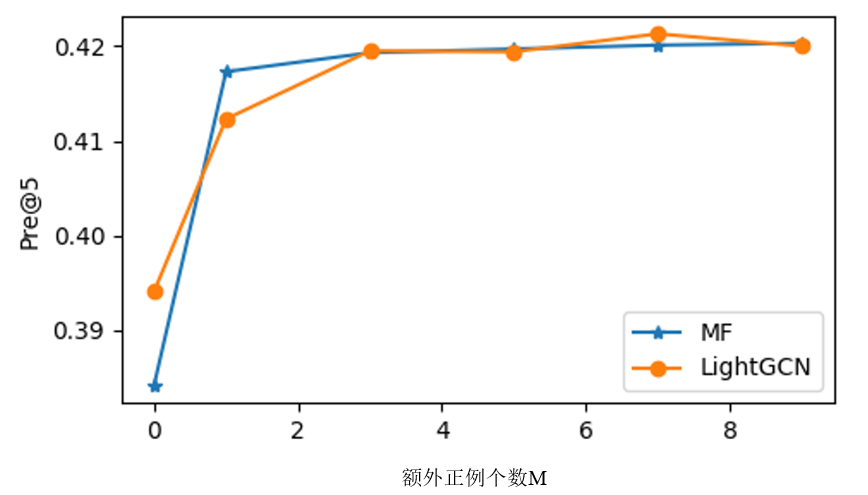
\includegraphics[width=0.7\textwidth]{4-parameter1.png}
	\caption{超参数M的影响}
	\label{Fig:parameter1}
\end{figure*}

\textbf{M参数的影响}:参数M控制用于纠正采样偏差的额外正例数量。当M=0时,没有去偏机制。当M$\geq$1时,DPL算法的去偏机制开始发挥最用,通过减去正例-正例对构造的伪AUC,得到正例-负例对构造的AUC优化目标,如图\ref{fig:auc}所示。
对于MF和LightGCN模型,较大的M和N导致性能提升,如图\ref{Fig:parameter1}所示。其中从M=0到M=1性能提升很显著,突出了使用额外正例进行去偏的重要性。然而,当M和N超过一个小的常数时,性能不再提高。这是因为进一步增加M和N所带来的估计准确性的边际收益变得有限。

\begin{figure*}[h!]
	\centering
	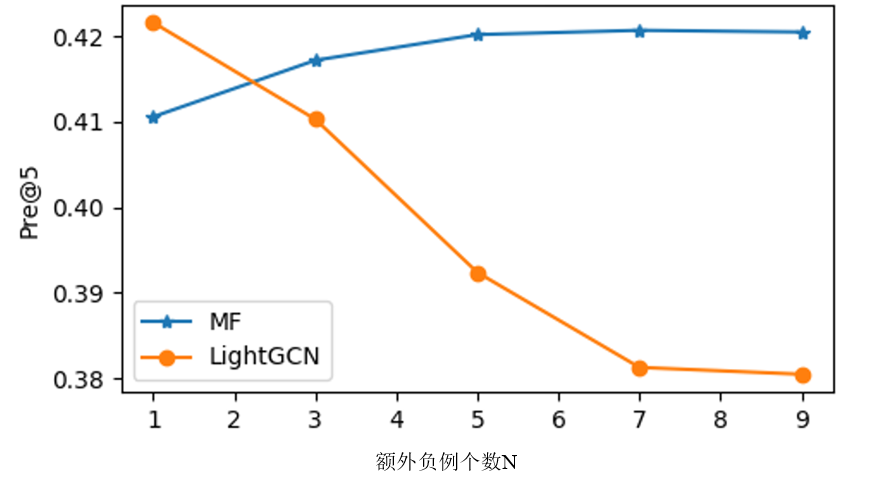
\includegraphics[width=0.7\textwidth]{4-parameter2.png}
	\caption{超参数N的影响}
	\label{Fig:parameter2}
\end{figure*}
\textbf{N参数的影响}:参数N控制用于计算PU概率的交互样本数量。对于MF模型,增加N会提高模型的性能。然而,对于LightGCN模型,当未标注样本数量N增加时,模型性下降。这个非预期的结果可能应该归因于较大的N会降低难负例样本的梯度值,从而削弱困难负样本对学习算法的贡献。根据DPL的损失计算方式,先计算PU概率的均值$\frac{1}{N} \sum_{i=1}^N P_n$,然后再取对数。然而,根据詹森不等式,$-\log(\frac{1}{N} \sum_{i=1}^N P_n) \leq -\frac{1}{N} \sum_{i=1}^N \log P_n $;因此,过高的N值削弱了困难负样本对学习算法的贡献。虽然本章的引理\ref{lemma:err}分析了估计误差随着N的增加而减小,但前提是得分$g(\cdot)$是独立同分布变量。然而,基于图神经网络编码器的聚合机制严重影响了$g(\cdot)$值的独立同分布性质。因此,当推荐模型为难以优化的神经网络模型如LightGCN时,应当设置较小的未标注样本个数N,以防止过大的N削弱了困难样本的贡献,从而对推荐性能产生不利影响。

\begin{figure*}[h!]
	\centering
	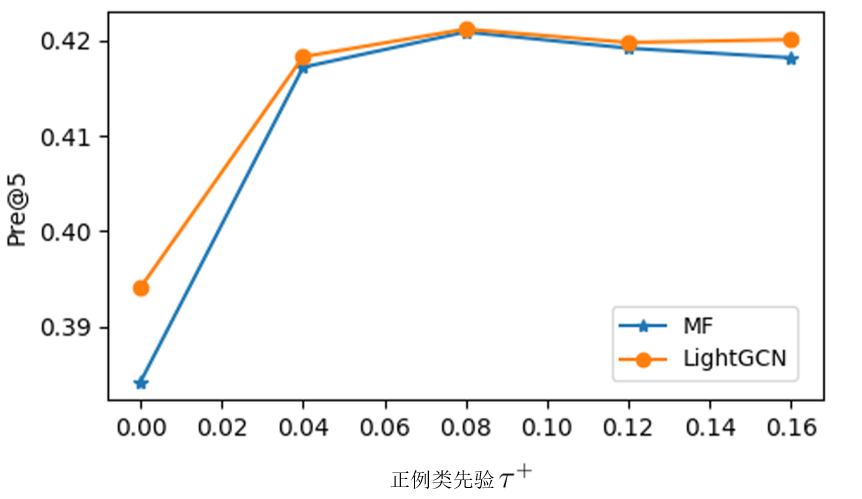
\includegraphics[width=0.7\textwidth]{4-parameter3.png}
	\caption{超参数$\tau^+$的影响}
	\label{Fig:parameter3}
\end{figure*}
\textbf{正类先验$\tau^+$的影响}:随着$\tau^+$增加或减少,MF和LightGCN模型的性能呈现出倒U型曲线,先增加后减少。特别地,当$\tau^+=0$时,DPL算法的去偏机制不发挥作用,因为$\tau^+=0$导致额外校正项等于0。当$\tau^+>0$时,MF和LightGCN模型性能都显著提升,也印证了去偏机制的重要性。但是当$\tau^+$大于0.08时,MF和LightGCN模型性能都出现了不同程度的下降。这是因为设置过低或过高的$\tau^+$值可能导致公式\eqref{eq:est}的估计结果偏差。

一种常见的设置$\tau^+$值的方法是将观察到数据集的交互数量$|\mathcal{D}^+|$视为伯努利试验的结果,对于$|\mathcal{U}|$个用户$|\mathcal{I}|$个物品的数据集,每次实验成功的概率为$\tau^+$,试验总共发生$|\mathcal{U}|\times |\mathcal{I}|$次,成功的次数为观察到的交互总数$|\mathcal{D}^+|$。因此,$|\mathcal{D}^+|/(|\mathcal{U}|\times |\mathcal{I}|)$可以作为设置$\tau^+$值的参考,其含义为数据集的密度。然而,需要注意的是,基于数据集密度设置的$\tau^+$值也是一种有偏估计,低估了真实值。这是因为数据中的所有未产生交互的样本对都被视为负样本,导致成功次数的低估,这也是MovieLens100K数据集的密度为0.06,而最优的$\tau^+$值在0.08左右取到的原因,最优的$\tau^+$值略大于数据集本身的密度。关于正例类先验的估计方法,详细讨论可参考~\cite{Jain:2016:NIPS,Christoffel:2016:ACML}。


\subsubsection{估计校正 vs 负采样}
负采样和估计校正代表了解决成对损失优化目标偏差问题的两种不同技术路径。负采样的核心思想是在模型外选择理想的样本并将其喂入模型训练;而估计校正的思想是使用随机样本,但对损失函数进行修正。从贝叶斯统计的角度来看,负采样利用了两种类型的信息:先验信息,如物品类别和流行度,这是静态的信息,用于采样用户不喜欢的负样本;样本信息,如分数和排名位置,这是动态的信息,在模型训练过程中不断调整,并用于采样困难(得分较高)样本。各种负采样算法之间的差异在于它们如何利用和处理这两种类型的信息。上一章的贝叶斯负采样算法提出了后验概率意义上的负信号测度,并指定了理论上最优的负采样准则。本节探讨估计校正和负采样这两种技术路径的优劣。
\begin{table*}[h!]
	\centering
	\caption{去偏成对学习算法与负采样算法的性能比较}\label{Table:vsns}
	\resizebox{1\textwidth}{!}{
		\begin{tabular}{lllccccccccccc}
			\toprule[1.2pt]
			\multirow{2}*{\textbf{数据集}} & \multirow{2}*{\textbf{推荐模型}} & \multirow{2}*{\textbf{方法}} & \multicolumn{3}{c}{Top-5} &~& \multicolumn{3}{c}{Top-10}&~&\multicolumn{3}{c}{Top-20}\\ \cline{4-6} \cline{8-10} \cline{12-14}
			~ & ~ & ~ & Precision& Recall& NDCG& ~ &Precision& Recall& NDCG& ~ &Precision& Recall& NDCG \\ \hline
			
			\multirow{4}*{\textbf{MovieLens-100k}} & \multirow{4}*{\textbf{MF}} & BPR & 0.3900   &0.1301	&0.4143	&~&0.3363	&0.2164	&0.3967& ~&0.2724&0.3298&0.3962 \\
			~ & ~ &BNS   &0.4205 &0.1467	&0.4558&~	&0.3463	&0.2290	&0.4217& ~&0.2762&0.3466& 0.4176\\	
			~ & ~ &DPL(Proposed)    &0.4348 & 0.1523 & 0.4643 & ~ & 0.3635 & 0.2379 & 0.4356 & ~ & 0.2914 & 0.3588 & 0.4338 \\
			~ & ~ &DPL with Hard Samples   &0.4401 & 0.1579 & 0.4692 & ~ & 0.3713 & 0.2407 & 0.4395 & ~ & 0.2940 & 0.3592 & 0.4351 \\\hline \hline 
			
			
			\multirow{4}*{\textbf{MovieLens-1M}} & \multirow{4}*{\textbf{MF}} & BPR &0.3843    &0.0855	&0.4027	&~&0.3353	&0.1430	&0.3737& ~&0.2798&0.2244&0.3572\\ 
			~ & ~ & BNS&0.4207	&0.1062	&0.4324&~	&0.3518	&0.1703	&0.4191& ~&0.3045&0.2614&0.4002 \\
			~ & ~ & DPL(proposed) & 0.4212 & 0.0998 & 0.4407 & ~ & 0.3624 & 0.1625 & 0.4071 & ~ & 0.2991 & 0.2518 & 0.3891  \\
			~ & ~ & DPL with Hard Samples & 0.4251 & 0.1012 & 0.4412 & ~ & 0.3649 & 0.1701 & 0.4151 & ~ & 0.3012 & 0.2539 & 0.3922  \\\hline 
			\bottomrule[1.5pt]
		\end{tabular}
	}
\end{table*}
\begin{figure}[h!]
	\centering
	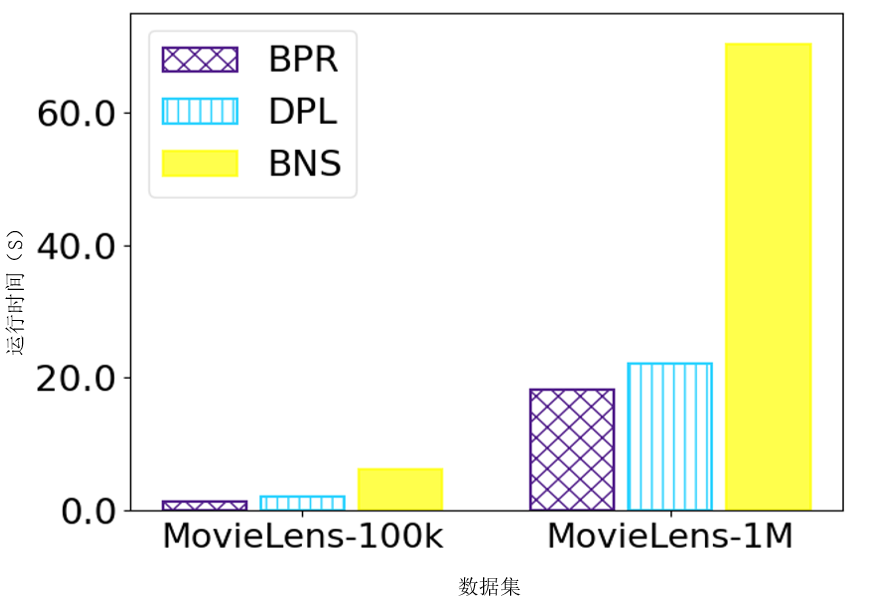
\includegraphics[width=0.7\textwidth]{4-runtime.png}
	\caption{去偏成对学习算法和负采样算法的运行时间比较} 
	\label{Fig:runtime}
\end{figure}

\textbf{性能比较}:
表~\ref{Table:vsns}中比较了DPL和BNS的性能。可以看到,DPL在MovieLens100k数据集上取得了更好的性能,并且在MovieLens1M数据集上与BNS表现相当,相对于BPR都取得了显著的提升,这表明基于校正估计的DPL和基于负采样的BNS都是有效的。此外,发现使用困难样本来训练DPL(标记为 DPL with Hard Samples)可以带来进一步的性能提升。当使用困难样本训练DPL时,需要设置相对较大的$\tau^+$值。在表~\ref{Table:vsns}中,分别将$\tau^+$设置为0.3和0.25,这比数据集本身的密度要高得多。这是因为使用困难样本训练DPL会增加模型遇到误分类负样本的概率,这相当于人为地改变了喂入模型的训练样本的正类先验概率。

\textbf{运行时间}: 运行时间是在一台配备2.1 GHz CPU、RTX 1080Ti GPU和32 GB RAM的个人计算机上进行测试的。图~\ref{Fig:runtime}显示了三种算法在五个数据集上进行一个训练轮次(Epoch)的实际运行时间,其中协同过滤模型固定为MF,批大小固定为1024。在计算经验分布函数时,BNS只采用mini-batch内的样本近似计算。如图~\ref{Fig:runtime}所示,DPL的实际运行时间仅略长于BPR,这与之前的时间复杂性分析一致。相对于BNS,即使采用mini-batch内的样本近似以节省计算成本,BNS的运行时间仍然是BPR和DPL的3-5倍。这是因为动态负采样需要预测得分来指导负采样,但基于GPU的批计算在进行前向传播以预测得分之前需要固定负样本。因此,动态负采样通常通过将额外的负样本作为候选项加载到小批量数据中来实现,从而导致额外的计算成本。此外,一些最先进的动态负采样算法根据前几个训练epoch中的样本预测得分计算方差~\cite{Ding:2019:NeurIPS},这要求模型在进行前向传播时计算整个用户-物品评分矩阵的预测得分,而不仅仅是mini-batch内样本的得分,从而导致时间复杂度的增加。

需要强调的是,负采样算法具有很好的灵活性,尤其是在有丰富的辅助信息用于监督的情况下,可以灵活地采样真负例和困难样本,而基于估计校正的方法难以做到这一点。总之,在具有丰富的辅助信息的场景中,建议使用可以灵活组合先验信息和模型信息的负采样算法。在没有可用的辅助信息进行监督的场景中,建议使用DPL方法进行损失修正。

\section{本章小结}
本章聚焦于正例-未标记(PU)的隐式反馈数据所造成的成对损失优化目标偏差问题,提出了基于成对损失的估计校正方法,从而为成对学习提供了一种修正的损失函数,称为去偏对数损失(Debiased Pairwise Loss,DPL)。DPL的关键思想是校正由伪负例导致的概率估计偏差,从而修正梯度以近似完全监督数据的梯度。所提出的目标函数易于实现,不需要额外的辅助信息进行监督,也不需要过多的存储和计算开销。在保持严格的相对于BPR的线性时间复杂度情况下,DPL取得了相对于负采样相当或更优的表现。

式\eqref{eq:infonce1}展示了成对损失和对比损失的联系,成对损失函数是负例个数N=1的对比损失的特例。本章聚焦于成对损失的去偏研究,DPL的去偏机制的核心可以参考图~\ref{fig:event},在只有一个负例的情况下,未标注样本的真实标签有且只有两种可能性,很容易被枚举出来。在自监督对比学习中,一个广泛的共识是负例个数N越大,学到的对比表示在下游任务中泛化表现越好\cite{Oord:2018:arxiv,Chuang:2020:NIPS,Robinson:2021:ICLR},这是由于更大的N推高了已知数据和待预测数据互信息的下界\cite{Oord:2018:arxiv}。但是,随着未标注样本N的增长,真实的标签的可能性指数级增长为$2^N$种,难以被枚举出来,导致本章的去偏思路则难以向更大的负例数推广。那么如何将去偏方法向多个负例的更一般的对比损失推广?此外,对于在自监督对比学习任务而言,除了去偏以保持正例的对齐性(即,防止用户喜欢的物品被推远),还有一个重要的硬负例挖掘任务(即,推远用户不喜欢的困难负例),以保持负例的均匀性\cite{Wang:2020:ICML,Feng:2021:CVPR}。本章只考虑到了前者。如何同时兼顾伪负例去偏和硬负例挖掘这两个矛盾的任务?下一个章节将针对这两个问题给出解决方案。

